\documentclass[useAMS, usenatbib, a4paper]{mnras}
\pdfsuppresswarningpagegroup=1

\usepackage{graphicx}
\usepackage{microtype}
\usepackage{xcolor}
\usepackage{fixltx2e}
\usepackage{booktabs}
\usepackage{siunitx}
\sisetup{separate-uncertainty = true}
\usepackage{color}
\usepackage{enumerate}
\usepackage{pdflscape}
\usepackage{rotating}
\usepackage{xr-hyper}
\usepackage{hyperref}

\usepackage[T1]{fontenc} 
\usepackage[utf8]{inputenc}

% Fonts 
\usepackage{newtxtext}
% Note: newtxmath must come AFTER newtxtext
\usepackage[varvw,smallerops]{newtxmath}

\usepackage{chemgreek}
\activatechemgreekmapping{newtx}
\usepackage{listings}

\hypersetup{colorlinks=True, linkcolor=blue!50!black, citecolor=black,
  urlcolor=blue!50!black}

\usepackage{etoolbox}
\robustify\bfseries
\robustify\itshape

%% The following hack solves a problem with
%% ERROR: \pdfendlink ended up in different nesting level than \pdfstartlink.
%% See https://tex.stackexchange.com/a/249743
\makeatletter
\patchcmd\@combinedblfloats{\box\@outputbox}{\unvbox\@outputbox}{}{%
  \errmessage{\noexpand\@combinedblfloats could not be patched}%
}%
\makeatother

%% Bold italic
\newcommand\hmmax{0}            % we don't need heavy fonts
\newcommand\bmmax{1}            % reduce use of math alphabets for bold
\usepackage{bm}

%% Bundled custom packages
\usepackage{aastex-compat}

\title
{Bow shocks, bow waves, and dust waves. I. Strong coupling limit}

\newcommand\AddressCRyA{Instituto de Radioastronom\'{\i}a y Astrof\'{\i}sica,
  Universidad Nacional Aut\'onoma de M\'exico, Apartado Postal 3-72,
  58090 Morelia, Michoac\'an, M\'exico}
\author[Henney \& Arthur]{
  William J. Henney \& S. J. Arthur\\
  \AddressCRyA
}

% These dates will be filled out by the publisher
\date{Accepted XXX. Received YYY; in original form ZZZ}

% Enter the current year, for the copyright statements etc.
\pubyear{2019}

\DeclareMathOperator{\sgn}{sgn}
\DeclareMathOperator{\Sin}{\mathcal{S}}
\DeclareMathOperator{\Cos}{\mathcal{C}}
\DeclareMathOperator{\Cot}{\mathcal{T}}
\DeclareMathOperator{\GammaFunc}{\Gamma}
\DeclareMathOperator\erf{erf}
\newcommand\w{\ensuremath{\mathrm{w}}}
\newcommand\C{\ensuremath{\mathrm{c}}}
\providecommand{\abs}[1]{\lvert#1\rvert}
\providecommand{\Abs}[1]{\left\lvert#1\right\rvert}
\newcommand\TODO[1]{%
  \begin{center}
    \framebox{\parbox{0.8\linewidth}{
        \texttt{\footnotesize\color{red} #1}}}
  \end{center}}

\newcommand\uvec[1]{\bm{\hat{#1}}}
\newcommand\T{_{\mathrm{\scriptscriptstyle T}}}

\newcommand\Qp{\ensuremath{Q_{\text{p}}}}
\newcommand\Qpbar{\ensuremath{\bar{Q}_{\text{p}}}}
\newcommand{\grain}{\ensuremath{_{\text{d}}}}
\newcommand{\B}{\ensuremath{_{\scriptscriptstyle\text{B}}}}
\newcommand{\alfven}{\ensuremath{_{\scriptscriptstyle\text{A}}}}
\newcommand{\xsec}{\ensuremath{\sigma\grain}}
\newcommand\frad{\ensuremath{f_{\text{rad}}}}
\newcommand\fmax{\ensuremath{f_{\text{max}}}}
\newcommand\thm{\ensuremath{\theta_{\text{m}}}}
\newcommand\drag{\ensuremath{_{\text{drag}}}}
\newcommand{\gas}{\ensuremath{_{\text{gas}}}}
\newcommand{\wind}{\ensuremath{_{\text{w}}}}
\newcommand{\trap}{\ensuremath{_{\text{abs}}}}
\newcommand{\ke}{\ensuremath{_{\text{kin}}}}
\newcommand{\drift}{\ensuremath{_{\text{drift}}}}
\newcommand\rad{\ensuremath{_{\text{rad}}}}
\newcommand\Lya{\ensuremath{_{\text{Ly}\alpha}}}
\newcommand\Rmin{\ensuremath{R_{\scriptscriptstyle\text{min}}}}
% Why do I need both of these?
\newcommand\sound{\ensuremath{c_{\text{s}}}}
\newcommand\soundspeed{\ensuremath{c_{\text{s,gas}}}}
\newcommand\starstar{\ensuremath{_{**}}}
\newcommand\mmp{\ensuremath{_{\text{\tiny MMP83}}}}
\newcommand\Hab{\ensuremath{_{\text{\tiny Habing}}}}
\newcommand\IR{\ensuremath{_{\text{IR}}}}
\newcommand{\thD}{\(\theta^1\)\,Ori~D}
\newcommand{\thC}{\(\theta^1\)\,Ori~C}
\newcommand\alphaB{\ensuremath{\alpha_{\text{B}}}}
\newcommand\shell{\ensuremath{_{\text{sh}}}}
\newcommand\M{\ensuremath{\mathcal{M}}}
\newcommand\hii{\ion{H}{ii}}

\newcommand\amu{\ensuremath{a_{\si{\um}}}}

\newcommand\freeze{\ensuremath{_{\text{tight}}}}
\newcommand\iftrap{\ensuremath{_{\text{trap}}}}
\newcommand\LOS{\ensuremath{_{\text{los}}}}


%%% Local Variables:
%%% mode: latex
%%% TeX-master: "bs-bw-dw-01"
%%% End:


% \externaldocument[Q-]{quadrics-bowshock}
% \externaldocument[II-]{bs-bw-dw-02}
% \externaldocument[III-]{bs-bw-dw-03}

\defcitealias{Tarango-Yong:2018a}{Paper~I}
\newcommand\PaperI{\citetalias{Tarango-Yong:2018a}}

\begin{document}
\label{firstpage}
\pagerange{\pageref{firstpage}--\pageref{lastpage}}
\maketitle
\begin{abstract}
  Dust waves and bow waves result from the action of a star's
  radiation pressure on a stream of dusty plasma that flows past it.
  They are an alternative mechanism to hydrodynamic bow shocks for
  explaining the curved arcs of infrared emission seen around some
  stars.  When gas and grains are perfectly coupled, for a broad class
  of stellar parameters, wind-supported bow shocks predominate when
  the ambient density is below \SI{100}{cm^{-3}}.  At higher densities
  radiation-supported bows can form, tending to be optically thin bow
  waves around B~stars, or optically thick bow shocks around early
  O~stars.  For OB stars with particularly weak stellar winds,
  radiation-supported bows become more prevalent.
\end{abstract}

\begin{keywords}
  circumstellar matter -- radiation: dynamics -- stars: winds, outflows
\end{keywords}

\defcitealias{Tarango-Yong:2018a}{Paper~I}
\newcommand\PaperI{\citetalias{Tarango-Yong:2018a}}

\section{Introduction}
\label{sec:introduction}
\newcommand\hii{\ion{H}{ii}}

Curved emission arcs around stars \citep[e.g.,][]{Gull:1979a} are
often interpreted as \textit{bow shocks}, due to a supersonic
hydrodynamic interaction between the star's wind and an external
stream. This stream may be due to the star's own motion or to an
independent flow, such as an \hii{} region in the champagne phase
\citep{Tenorio-Tagle:1979a}, or another star's wind
\citep{Canto:1996}. However, an alternative interpretation in some
cases may be a radiation-pressure driven bow wave, as first proposed
by \citet[\S\textsc{vi}]{van-Buren:1988a}.  In this scenario, photons
emitted by the star are absorbed by dust grains in the incoming
stream, with the resultant momentum transfer being sufficient to
decelerate and deflect the grains within a certain distance from the
star, forming a dust-free, bow-shaped cavity with an enhanced dust
density at its edge.  Two regimes are possible, depending on the
strength of coupling between the gas (or plasma) and the dust.  In the
strong-coupling regime, gas--grain drag decelerates the gas along with
the dust, forming a shocked gas shell in a similar fashion to the
wind-driven bow shock case.  In the weak-coupling regime, the gas
stream is relatively unaffected and the dust temporarily decouples to
form a dust-only shell.  This second case has recently been studied in
detail in the context of the interaction of late O-type stars (which
have only weak stellar winds) with dusty photoevaporation flows inside
\hii{} regions \citep{Ochsendorf:2014a, Ochsendorf:2014b,
  Ochsendorf:2015a}.  We follow the nomenclature proposed by
\citet{Ochsendorf:2014b}, in which \textit{dust wave} refers to the
weak coupling case and \textit{bow wave} to the strong coupling case.
More complex, hybrid scenarios are also possible, such as that studied
by \citet{van-Marle:2011a}, where a hydrodynamic bow shock forms, but
the larger dust grains that accompany the stellar wind pass right
through the shocked gas shell, and form their own dust wave at a
larger radius.

\begin{figure*}
  \centering
  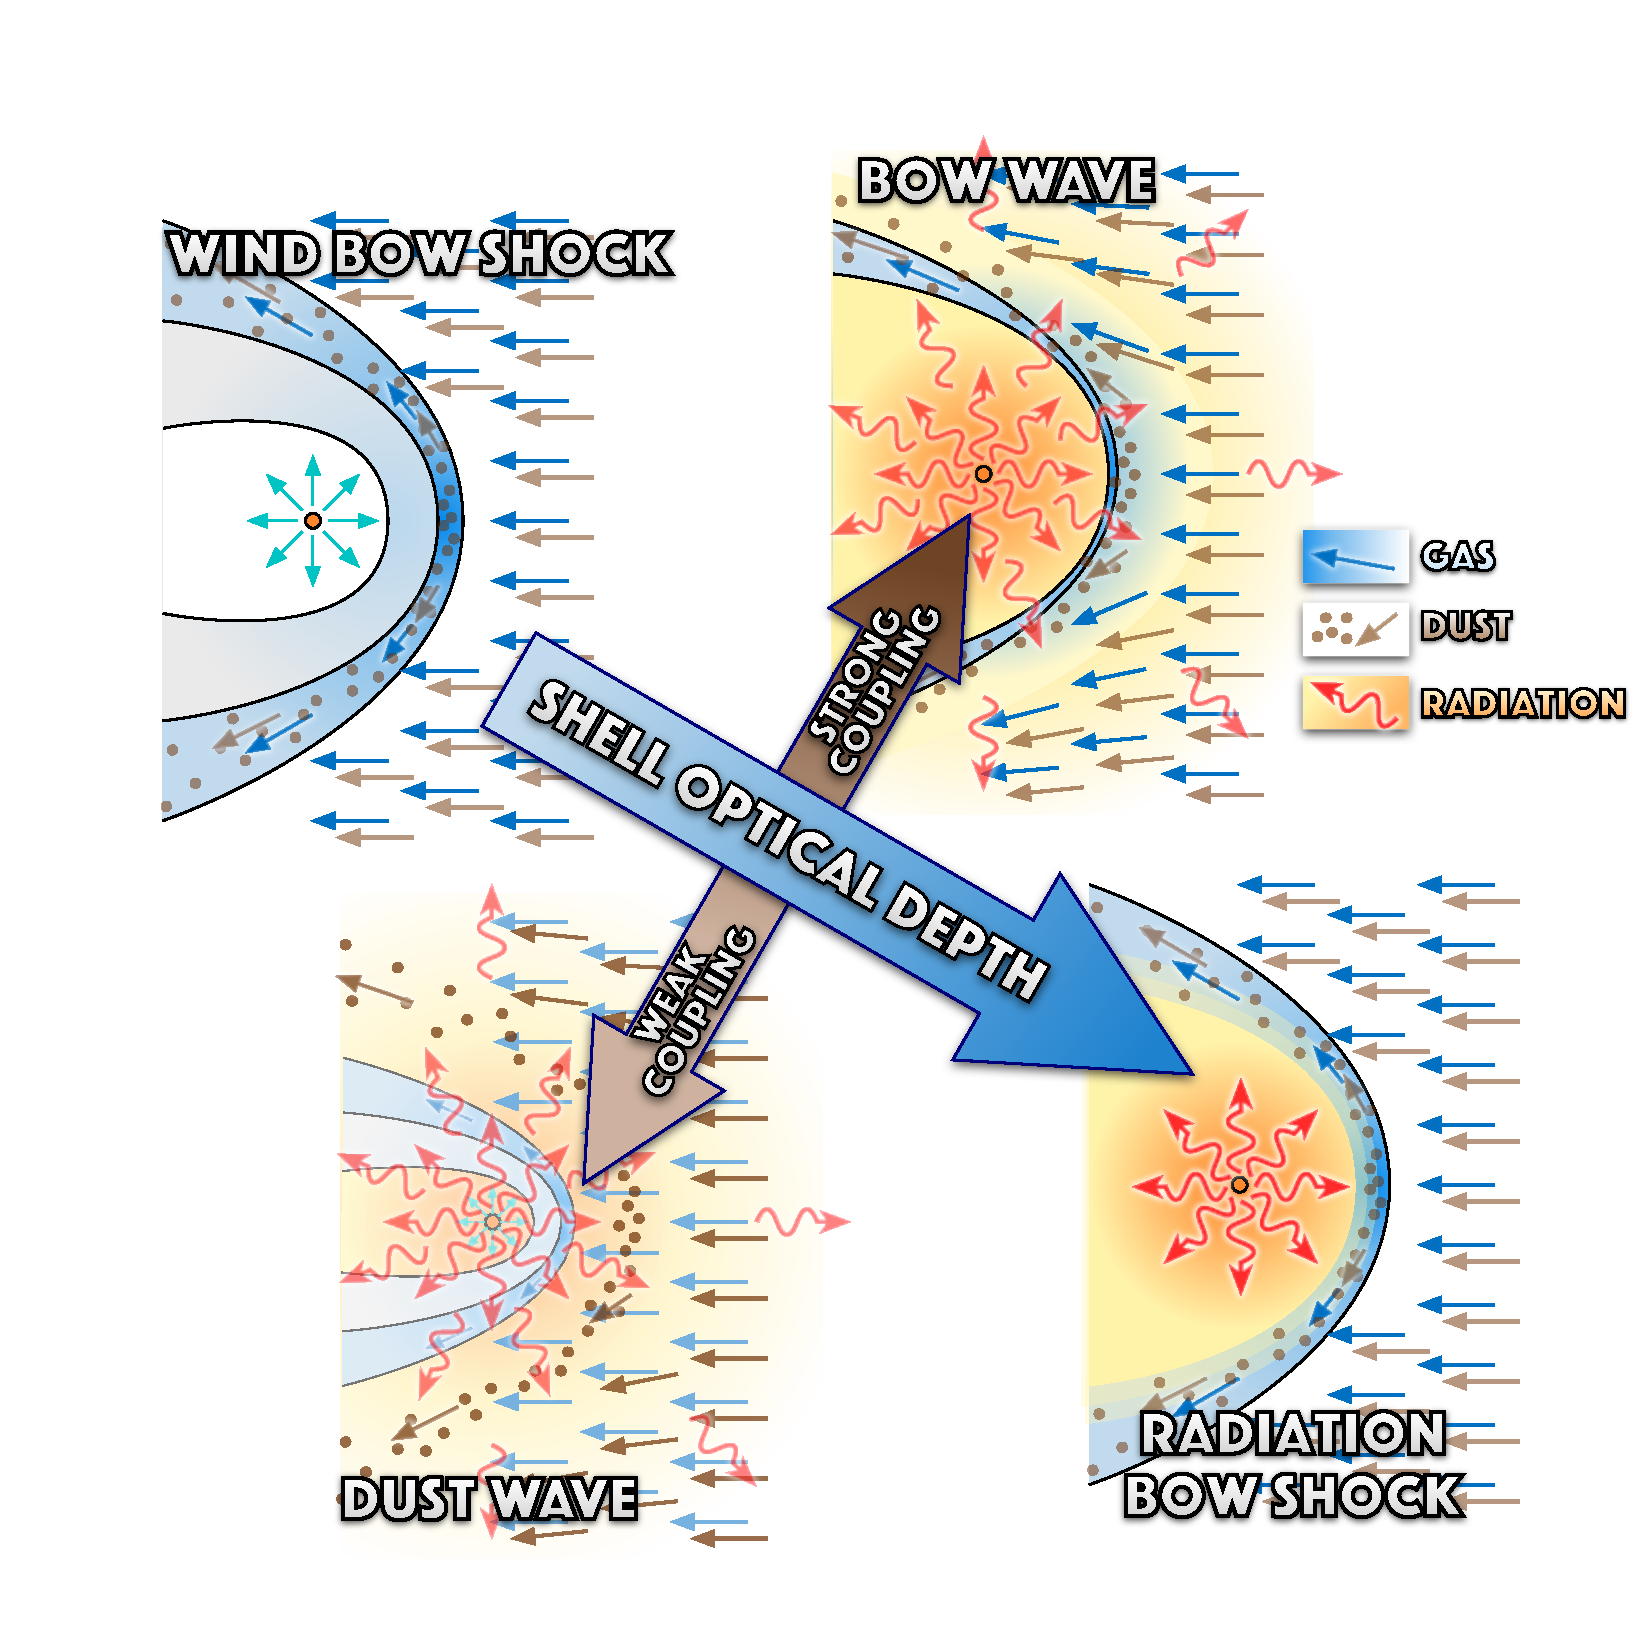
\includegraphics[width=\linewidth]{figs/bows-and-waves}
  \caption{Bow shocks, bow waves, and dust waves}
  \label{fig:3-types-bow}
\end{figure*}

In \citet[][hereafter \PaperI{}]{Tarango-Yong:2018a}, we proposed a
new two-dimensional classification scheme for bow shapes: the
projected planitude--alatude, or \(\Pi'\)--\(\Lambda'\), diagram.  Planitude
measures the flatness of the bow's apex, while alatude measures the
openness of the bow's wings.  Both are dimensionless ratios of lengths
that can be estimated from observational images.  We have analyzed the
inclination-dependent tracks on the \(\Pi'\)--\(\Lambda'\) plane for simple
geometric shapes (spheroids, paraboloids, hyperboloids) and for
thin-shell hydrodynamic bow shock models (wilkinoid, cantoids,
ancantoids).  In this paper, we will do the same for simple models of
radiation-driven dust waves (dragoids) and bow waves (trapoids).

The paper is organized as follows.
%
In \S~\ref{sec:shape-dust-wave} we do the same for simple models of a
dusty radiation bow wave (dragoids), including the effects of
gas-grain drag.
%
In \S~\ref{sec:perturbed-bows} we investigate the effects on the
planitude--alatude plane of small-amplitude perturbations to the bow
shape.
%


\section{Different types of bow}
\label{sec:different-types-bow}

\begin{figure*}
  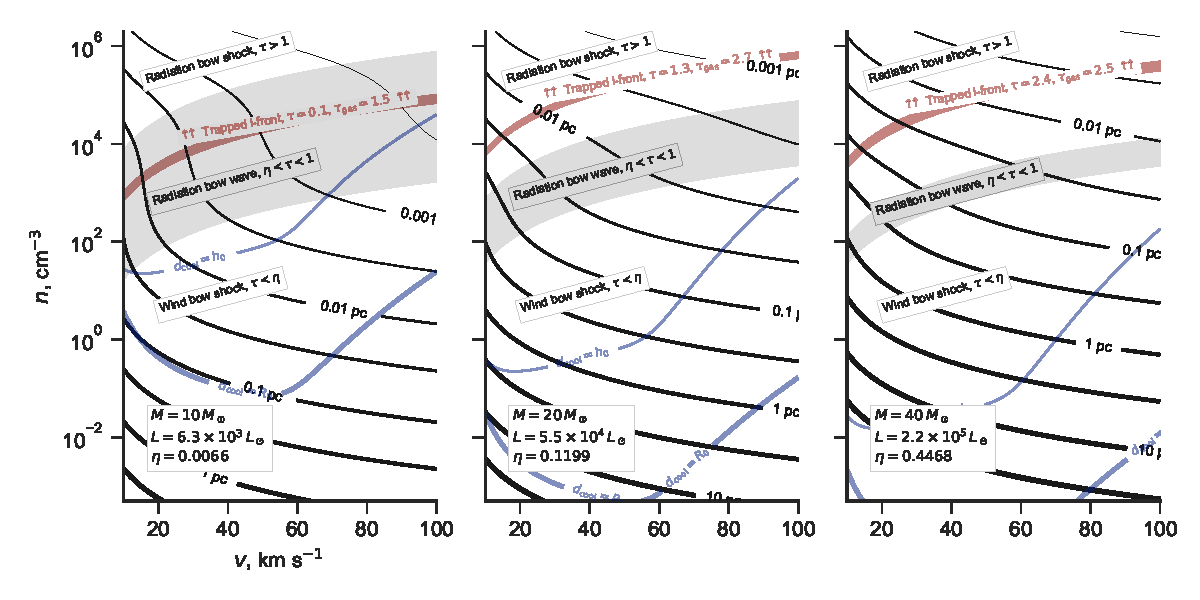
\includegraphics[width=\linewidth]{figs/zones-v-n-plane}
  \caption{Bow regimes in parameter space (\(v, n\)) of the external
    stream for main-sequence OB stars of different masses:
    (a)~\SI{10}{M_\odot}, (b)~\SI{20}{M_\odot}, (c)~\SI{40}{M_\odot}.  In all
    cases, \(\kappa = \SI{600}{cm^2.g^{-1}}\) and efficient gas-grain
    coupling is assumed. Solid black lines of varying width show the
    bow size (star-apex separation, \(R_0\)), while gray shading shows
    the radiation bow wave regime, with lower border \(\tau = \eta\) and
    upper border \(\tau = 1\), where \(\tau = 2 \kappa \rho R_0\) is the optical
    depth through the bow.  For bows above the red solid line, the
    ionization front is trapped inside the bow.  Blue lines delineate
    different cooling regimes.  Above the thin blue line
    (\(d_{\text{cool}} = h_0\)), the bow shock radiates efficiently,
    forming a thin shocked shell.  Below the thick blue line
    (\(d_{\text{cool}} = R_0\)), the bow shock is essentially
    non-radiative.}
  \label{fig:zones-v-n-plane}
\end{figure*}

In this section, we investigate the different types of bow interaction
that will occur in different regions of parameter space. We will
mainly treat the canonical case\footnote{%
  Variant cases with differing arrangements of dust and radiation
  sources are treated in \S~\ref{sec:case-inside-out}.} %
of a bow around a star of bolometric luminosity, \(L\), with a
radiatively driven wind, which is immersed in an external stream of
gas and dust with density, \(\rho\), and velocity, \(v\).  The size and
shape of the bow is determined by a generalized balance of pressure
(or, equivalently, momentum) between internal and external sources.
We assume that the stream is supersonic and super-alfvenic, so that
the external pressure is dominated by the ram pressure: \(\rho v^2\).

\subsection{Strong gas-grain coupling}
\label{sec:strong-gas-grain}

We first consider the case where the dust grains and gas are perfectly
coupled by collisions.\footnote{%
  Cases where this assumption does not hold are investigated below in
  \S~\ref{sec:imperf-coupl-betw}.} %
Although dust grains typically constitute only a small fraction
\(Z\grain \sim 0.01\) of the mass of the external stream, they
nevertheless dominate the broad-band opacity at FUV, optical and IR
wavelengths if they are present.\footnote{%
  At EUV wavelengths (\(\lambda < \SI{912}{\angstrom}\)), gas opacity
  dominates if the hydrogen neutral fraction is larger than
  \(\approx 0.001\), see discussion of ionization front trapping
  below.} %
The strong coupling assumption means that all the radiative forces
applied to the dust grains are directly felt by the gas also.

\subsubsection{Bows supported by radiation and wind}
\label{sec:three-bow-regimes}

The internal pressure is the sum of wind ram pressure and the
effective radiation pressure that acts on the bow shell.  The
radiative momentum loss rate of the star is \(L/c\) and the wind
momentum loss rate can be expressed as
\begin{equation}
  \label{eq:wind-efficiency}
  \dot{M} V = \eta L / c \ , 
\end{equation}
where \(\eta\) is the momentum efficiency of the wind, which is typically
\(< 1\) \citep{Lamers:1999b}. If the optical depth is very large, then
all of the stellar radiative momentum, emitted with rate \(L/c\), is
trapped by the bow shell.  In the single scattering limit,\footnote{%
  Although it may seem inconsistent to assume single scattering in the
  case of high optical depths, this is defensible for the following
  reasons. (1)~The grain albedo is not that high (typically
  \(\sim 0.5\) at ultraviolet through optical wavelengths). (2)~The
  scattered radiation field is more isotropic than the stellar field,
  leading to cancellation in the radiative
  flux. (3)~Absorbed radiation is re-emitted at infrared
  wavelengths, where the dust opacity is very much lower.} %
and temporarily neglecting the wind, then pressure balance at the bow
apex, a distance \(R_0\) along the symmetry axis from the star is
given by
\begin{equation}
  \label{eq:rad-press-balance-thick}
  \frac{L}{4 \pi c R_0^2} = \rho v^2 \ ,
\end{equation}
which yields a fiducial bow shock radius in this optically thick limit
as
\begin{equation}
  \label{eq:Rstar}
  R_* = \left(\frac{L}{4\pi c \rho v^2}\right)^{1/2} \ .
\end{equation}

We now consider the opposite, optically thin limit.  If the total
opacity (gas plus dust) per total mass (gas plus dust) is \(\kappa\) (with
units of \si{cm^2.g^{-1}}), then the radiative acceleration is
\begin{equation}
  \label{eq:rad-accel}
  a_{\text{rad}} = \frac{\kappa L}{4 \pi c R^2} \ .
\end{equation}
Therefore, an incoming stream with initial velocity, \(v_\infty\), can be
brought to rest by radiation alone\footnote{%
  For simplicity, we here ignore the effects of gravity, which are
  important for low ratios of \(\kappa L / M\), see
  \S~\ref{sec:effects-gravity}.  We also ignore pressure gradients and
  shocks, which are important as the velocity approaches the sound
  speed, \(\sound\) (in \S~XX below, we show that the resultant
  corrections to \(R_0\) are of order \(\sound / v_\infty\)).} %
at a distance \(R_0\) where
\begin{equation}
  \label{eq:rad-poten}
  \int_{R_0}^\infty a_{\text{rad}} \, dr = \tfrac12 v_\infty^2 \ , 
\end{equation}
yielding
\begin{equation}
  \label{eq:rad:R0}
  R_0 = \frac{\kappa L}{2\pi c v_\infty^2} \ .
\end{equation}
On the other hand, we can also argue as in the optically thick case
above by approximating the bow shell as a surface, and balancing
stellar radiation pressure against the ram pressure of the incoming
stream.  The important difference when the shell is not optically
thick is that only a fraction \(1 - e^{-\tau}\) of the radiative momentum
is absorbed by the bow, so that
equation~\eqref{eq:rad-press-balance-thick} is replaced with
\begin{equation}
  \label{eq:rad-press-balance-tau}
  \frac{L (1 - e^{-\tau})}{4 \pi c R_0^2} = \rho v^2 \ .
\end{equation}
In the optically thin limit, \(1 - e^{-\tau} \approx \tau\), so these two
descriptions can be seen to agree so long as
\begin{equation}
  \label{eq:tau-thin}
  \tau = 2 \kappa \rho R_0 \ ,
\end{equation}
which we will assume to hold generally.

Then, defining a fiducial optical depth,
\begin{equation}
  \label{eq:tau-star}
  \tau_* = \rho \kappa R_* \ ,
\end{equation}
and adding in the stellar wind ram pressure\footnote{%
  We implicitly assume that the interaction of the stellar wind with
  the external stream can always be treated in the continuum limit.
  This will be true if either the collisional mean free path or the
  ion Larmor radius is much smaller than \(R_0\), which is almost
  always the case.} %
from equation~\eqref{eq:wind-efficiency}, we find that the general bow
radius can be written in terms of the fiducial radius as
\(R_0 = x R_*\), where \(x\) is the solution of
\begin{equation}
  \label{eq:rad-full-x}
  x^2 - \bigl(1 - e^{-2 \tau_* x} \bigr) - \eta = 0 \ .
\end{equation}
Since this is a transcendental equation, \(x\) must be found
numerically, but we can write explicit expressions for three limiting
cases:
\begin{equation}
  \label{eq:x-cases}
  x \approx
  \begin{cases}
    \text{if \(\tau_* \gg 1\):} & (1 + \eta)^{1/2}  \\
    \text{if \(\tau_*^2 \ll 1\):} & \tau_* + \bigl( \tau_*^2 + \eta \bigr)^{1/2} \approx
    \begin{cases}
      \text{if \(\tau_*^2 \gg \eta\):} & 2 \tau_*  \\
      \text{if \(\tau_*^2 \ll \eta\):} & \eta^{1/2} 
    \end{cases}
  \end{cases}
\end{equation}
The first case, \(x \approx (1 + \eta)^{1/2}\), corresponds to a
\textit{radiation bow shock}; the second case,
\(x \approx 2 \tau_* \), corresponds to a \textit{radiation bow wave}; and the
third case, \(x \approx \eta^{1/2}\), corresponds to a \textit{wind bow shock}.
The two bow shock cases are similar in that the external stream is
oblivious to the presence of the star until it suddenly hits the bow
shock shell, differing only in whether it is radiation or wind that is
providing the internal pressure.  In the intermediate bow wave case,
on the other hand, the external stream is gradually decelerated by
absorption of photons as it approaches the bow.\footnote{A shock does
  still form in this case, but shocked material constitutes only a
  fraction of the total column density of the shell, see
  \S~\ref{sec:shape-bow-wave}.}

\begin{table*}
  \centering
  \caption{Stellar parameters for example stars}
  \label{tab:stars}
  \begin{tabular}{l S S S S S S S S S l}
    \toprule
    & {\(M / \si{M_\odot}\)} & {\(L_4\)}
    & {\(\dot{M}_{-7}\)} & {\(V_3\)} & {\( \eta \)}
    & {Sp.~Type} 
    & {\(T_{\text{eff}} / \si{kK}\)} & {\(\lambda_{\text{eff}}\) / \si{\um}}
    & {\(S_{49}\)} & Figures 
    \\
    \midrule
    & 10 & 0.63 & 0.0034 & 2.47 & 0.0066 & {B1.5\,V} & 25.2 & 0.115 & 0.00013
                   & \ref{fig:zones-v-n-plane}a,
                     \ref{fig:decouple-v-n-plane},
                     \ref{fig:decouple-v40-versus-n} \\
    Main-sequence OB stars
    & 20 & 5.45 & 0.492 & 2.66 & 0.1199 & {O9\,V} & 33.9 & 0.086 & 0.16
                   & \ref{fig:zones-v-n-plane}b\\
    & 40 & 22.2 & 5.1 & 3.31 & 0.4468 & {O5\,V} & 42.5 & 0.068 & 1.41
                   & \ref{fig:zones-v-n-plane}c\\[\smallskipamount]
    Blue supergiant star
    & 33 & 30.2 & 20.2 & 0.93 & 0.3079 & {B0.7\,Ia} & 23.5 & 0.123 & 0.016
                   & \ref{fig:B-supergiant} \\[\smallskipamount]
    Red supergiant star
    & 20 & 15.6 & 100 & 0.015 & 0.0476 & {M1\,Ia} & 3.6 & 0.805 & 0
                   & \ref{fig:M-supergiant} \\ 
    \bottomrule
  \end{tabular}
\end{table*}

We now consider the application to bow shocks around main sequence OB
stars, expressing stellar and ambient parameters in terms of typical
values as follows:
\begin{align*}
  \label{eq:stellar-parameters}
  \dot{M}_{-7} &= \dot{M} / \bigl(\SI{e-7}{M_\odot.yr^{-1}}\bigr) \\
  V_3 &= V / \bigl(\SI{1000}{km.s^{-1}}\bigr) \\
  L_4 &= L / \bigl(\SI{e4}{L_\odot}\bigr) \\
  v_{10} &= v_\infty / \bigl( \SI{10}{km.s^{-1}} \bigr) \\
  n &= (\rho / \bar{m}) / \bigl( \SI{1}{cm^{-3}} \bigr) \\
  \kappa_{600} &= \kappa / \bigl( \SI{600}{cm^2.g^{-1}} \bigr) \ ,
\end{align*}
where \(\bar{m}\) is the mean mass per hydrogen nucleon
(\(\bar{m} \approx 1.3 m_{\text{p}} \approx \SI{2.17e-24}{g}\) for solar
abundances).  Note that \(\kappa = \SI{600}{cm^2.g^{-1}}\) corresponds to a
cross section of \(\approx \SI{e-21}{cm^2}\) per hydrogen nucleon, which is
typical for interstellar medium dust \citep{Bertoldi:1996a} at far
ultraviolet wavelengths, where OB stars emit most of their radiation.
In terms of these parameters, we can express the stellar wind momentum
efficiency as
\begin{equation}
  \label{eq:wind-eta-typical}
  \eta = \num{0.495} \,\dot{M}_{-7} \,V_3  \,L_4^{-1}
\end{equation}
and the fiducial radius and optical depth as
\begin{align}
  \label{eq:Rstar-typical}
  R_* / \si{pc} &= \num{2.21} \, (L_4 / n)^{1/2} \,v_{10}^{-1} \\
  \label{eq:taustar-typical}
  \tau_* &= \num{0.0089} \,\kappa_{600} \, (L_4 \,n)^{1/2} \,v_{10}^{-1} \ .
\end{align}
In Figure~\ref{fig:zones-v-n-plane}, we show results for the bow size
(apex distance, \(R_0\)) as a function of the density, \(n\), and
relative velocity, \(v_\infty\), of the external stream, with each panel
corresponding to a particular star, with parameters as shown in
Table~\ref{tab:stars}.  To facilitate comparison with previous work,
we choose stellar parameters similar to those used in the
hydrodynamical simulations of \citet{Meyer:2014b, Meyer:2016a,
  Meyer:2017a}, based on stellar evolution tracks for stars of
\SIlist{10;20;40}{M_\odot} \citep{Brott:2011a} and theoretical wind
prescriptions \citep{de-Jager:1988a, Vink:2000a}.  Although the
stellar parameters do evolve with time, they change relatively little
during the main-sequence lifetime of several million years.\footnote{%
  \label{fn:meyer-velocities-too-low}
  Note that we have recalculated the stellar wind terminal velocities,
  since the values given in the \citeauthor{Meyer:2014b} papers are
  troublingly low.  We have used the prescription
  \(V = 2.6 V_{\text{esc}}\), where
  \(V_{\text{esc}} = \left( 2 G M (1 - \Gamma_e)/ R \right)^{1/2}\) is the
  photospheric escape velocity, which is appropriate for strong
  line-driven winds with \(T_{\text{eff}} > \SI{21 000}{K}\)
  \citep{Lamers:1995a}.  We find velocities of
  \SIrange{2500}{3300}{km.s^{-1}}, which are consistent with
  observations and theory \citep{Vink:1999a} for O~stars, but at least
  two times higher than those cited by \citet{Meyer:2014b}. For
  main-sequence B~stars, wind column densities are too low to reliably
  measure the terminal velocity from near ultraviolet P~Cygni profiles
  \citep{Prinja:1989a}, and so the values are theory-dependent
  \citep{Krticka:2014a} and hence more uncertain.  A further
  complication is the existence of a subset of OB stars with
  anomalously weak winds \citep{Puls:2008a}, which in some cases is
  related to the presence of strong (\(\sim \SI{1}{kG}\)) magnetic fields
  \citep{Oskinova:2011b}.} %
The three examples are an early B~star (\SI{10}{M_\odot}), a late O~star
(\SI{20}{M_\odot}), and an early O~star (\SI{40}{M_\odot}), which cover the
range of luminosities and wind strengths expected from bow-producing
hot main sequence stars.  The luminosity is a steep function of
stellar mass (\(L \sim M^{2.5}\)) and the wind mass-loss rate is a steep
function of luminosity (\(\dot{M} \sim L^{2.2}\)), which means that the
wind momentum efficiency is also a steep function of mass
(\(\eta \sim M^3\)), approaching unity for early O~stars, but falling to
less than 1\% for B~stars.

\begin{figure}
  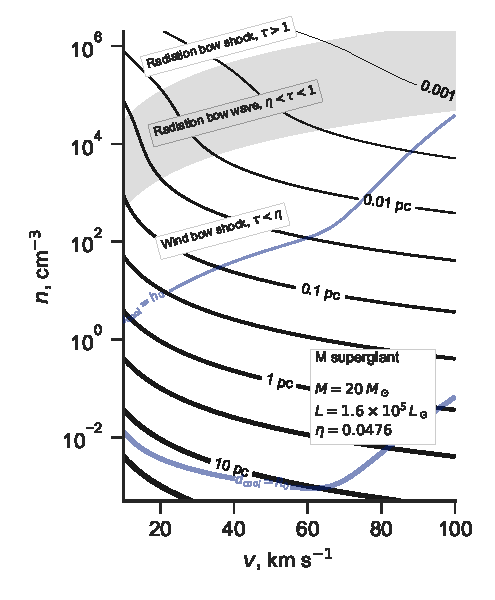
\includegraphics[width=\linewidth]{figs/zones-v-n-plane-RSG}
  \caption{As Fig.~\ref{fig:zones-v-n-plane}, but for a cool M-type
    supergiant instead of hot main sequence stars.  A smaller dust
    opacity is used, \(\kappa = \SI{60}{cm^2.g^{-1}}\), because of the
    reduced extinction efficiency at the optical/infrared wavelengths
    emitted by this star.}
  \label{fig:M-supergiant}
\end{figure}

It can be seen from Figure~\ref{fig:zones-v-n-plane} that the onset of
the radiation bow wave regime is very similar for the three
main-sequence stars, occurring at
\(n > \text{\numrange{20}{40}} \, v_{10}^2\).  An important
difference, however, is that for the \SI{40}{M_\odot} star, which has a
powerful wind, the radiation bow wave regime only occurs for a very
narrow range of densities, whereas for the \SI{10}{M_\odot} star, with a
much weaker wind, the regime is much broader, extending to
\(n < \num{e4} \, v_{10}^2\).  Another difference is the size scale of
the bows in this regime, which is
\(R_0 = \text{\SIrange{0.001}{0.003}{pc}}\) for the \SI{10}{M_\odot} star
if \(v_\infty = \SI{40}{km.s^{-1}}\), but \(R_0 \approx \SI{0.1}{pc}\) for the
\SI{40}{M_\odot} star, assuming the same inflow velocity.

Figure~\ref{fig:M-supergiant} shows results for a cool M-type
super-giant star with stellar parameters inspired by Betelgeuse
(\chemalpha~Orionis), as listed in Table~\ref{tab:stars}.  Unlike the
UV-dominated spectrum of the hot stars, this star emits predominantly
in the near-infrared, where the dust extinction efficiency is lower,
so we adopt a lower opacity of \SI{60}{cm^2.g^{-1}}.  This has the
effect of shifting the radiation bow wave regime to higher densities:
\(n = \text{\numrange{1000}{30 000}}\, v_{10}^2\) in this case.


\subsubsection{Effects of stellar gravity}
\label{sec:effects-gravity}

In principle, gravitational attraction from the star, of mass \(M\),
will partially counteract the radiative acceleration.  This can be
accounted for by replacing \(L\) with an effective luminosity
\newcommand\Edd{\ensuremath{_{\text{E}}}}
\begin{equation}
  \label{eq:effective-luminosity}
  L_{\text{eff}} = L \bigl(1 - \Gamma\Edd^{\,-1}\bigr) \ ,
\end{equation}
in which \(\Gamma\Edd\) is the Eddington factor:
\begin{equation}
  \label{eq:eddington-factor}
  \Gamma\Edd = \frac{\kappa L}{4\pi c G M} = 458.5 \, \frac{\kappa_{600} L_4}{ M } \ ,
\end{equation}
where, in the last expression, \(M\) is measured in solar masses.  For
the stars in Table~\ref{tab:stars}, we find
\(\Gamma\Edd \approx \text{\numrange{30}{400}}\), so gravity can be safely
ignored.  The only exception is when the optical depth of the bow is
very large: \(\tau > \ln\Gamma\Edd \sim 5\), in which case gravity may be
important in the outer parts of the shell (see
\citealt{Rodriguez-Ramirez:2016b}).



\subsubsection{Ionization state of the bow shell}
\label{sec:trapp-ioniz-front}

\newcommand\alphaB{\ensuremath{\alpha_{\text{B}}}}
\newcommand\shell{\ensuremath{_{\text{sh}}}}

\begin{figure}
  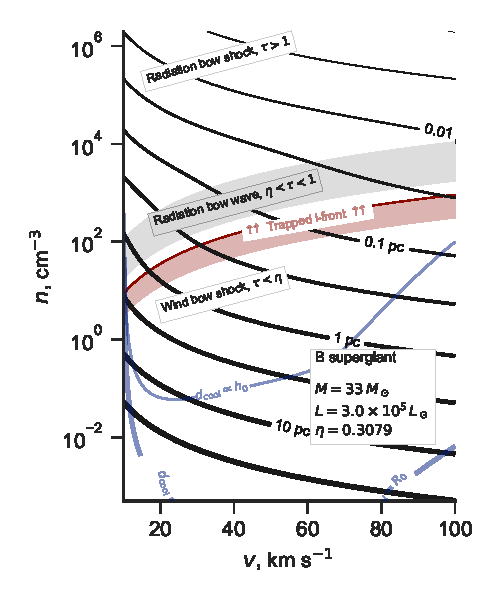
\includegraphics[width=\linewidth]{figs/zones-v-n-plane-BSG}
  \caption{As Fig.~\ref{fig:zones-v-n-plane}, but for an evolved
    B-type supergiant instead of main sequence stars.  This is similar
    to the early O MS star of Fig.~\ref{fig:zones-v-n-plane}\textit{c}
    in many respects, except for the trapping of the ionization front,
    which occurs for much lower outer stream densities.}
  \label{fig:B-supergiant}
\end{figure}

In this section we calculate whether the star is capable of
photoionizing the entire bow shock shell, or whether the ionization
front will be trapped within it.  The number of hydrogen
recombinations\footnote{%
  The diffuse field is treated in the on-the-spot approximation,
  assuming all emitted Lyman continuum photons are immediately
  re-absorbed locally, so the case~B recombination co-efficient,
  \(\alphaB = \num{2.6e-13}\, T_4^{-0.7}\, \si{cm^3.s^{-1}}\), is
  used, where \(T_4 = T/\SI{e4}{K}\).} %
per unit time per unit area in a fully ionized shell is
\begin{equation}
  \label{eq:shell-recombination-rate}
  \mathcal{R} = \alphaB n\shell^2 h\shell \ ,
\end{equation}
while the advective flux of hydrogen nuclei through the shock is 
\begin{equation}
  \label{eq:shell-advective-flux}
  \mathcal{A} = n v \ ,
\end{equation}
and the flux of hydrogen-ionizing photons
(\(h \nu > \SI{13.6}{eV}\)) incident on the inner edge of the shell is
\begin{equation}
  \label{eq:shell-ionizing-flux}
  \mathcal{F} = \frac{S} {4 \pi R_0^2} \ , 
\end{equation}
where \(S\) is the ionizing photon luminosity of the star.  Any shell
with \(\mathcal{R} + \mathcal{A} > \mathcal{F}\) cannot be entirely
photoionized by the star, and so must have trapped the ionization
front.

The ratio of advective particle flux to ionizing flux is, from
equations~\eqref{eq:Rstar}, \eqref{eq:shell-advective-flux},
\eqref{eq:shell-ionizing-flux},
\begin{equation}
  \label{eq:advective-over-ionizing-flux}
  \frac{\mathcal{A}}{\mathcal{F}} = \num{5.86e-5} \frac{x^2 L_4}{v_{10} S_{49}} \ , 
\end{equation}
which is nearly always small.  For clarity of exposition, we therefore
ignore \(\mathcal{A}\) in the following discussion, although it is
included in quantitative calculations.  The column density of the
shocked shell can be found, for example, from equations~(10) and~(12)
of \citet{Wilkin:1996a} in the limit \(v_\infty/V \to 0\) (Wilkin's parameter
\(\alpha\)) and \(\theta \to 0\).  This yields
\begin{equation}
  \label{eq:shocked-shell-column}
  n\shell h\shell = \tfrac34 n R_0 \ .
\end{equation}
Assuming strong cooling behind the shock,\footnote{%
  This is shown to be justified in \S~\ref{sec:radi-cool-lengths}.
} %
the shell density is
\begin{equation}
  \label{eq:isothermal-shell-density}
  n\shell = \mathcal{M}_0^2 n \,
\end{equation}
where
\(\mathcal{M}_0 = v_\infty / \sound\) is the isothermal Mach number of the
external stream.\footnote{%
  \label{fn:temperature-dependence}
  The sound speed depends on the temperature and hydrogen and helium
  ionization fractions, \(y\) and \(y_{\text{He}}\) as
  \(\sound^2 = (1 + y + z_{\text{He}} y_{\text{He}}) (k T /
  \bar{m})\), where \(z_{\text{He}}\) is the helium nucleon abundance
  by number relative to hydrogen and
  \(k = \SI{1.3806503e-16}{erg.K^{-1}}\) is Boltzmann's constant.  We
  assume \(y = 1\), \(y_{\text{He}} = 0.5\), \(z_{\text{He}} = 0.09\),
  so that \(\sound = \num{11.4}\, T_4^{1/2}\, \si{km.s^{-1}}\). } %
Putting these together with equations~\eqref{eq:Rstar} and
~\eqref{eq:tau-star}, one finds that \(\mathcal{R} > \mathcal{F}\)
implies
\begin{equation}
  \label{eq:ifront-trap-x-cubed-taustar}
  x^3 \tau_* > \frac{4 S c \sound \bar{m}^2 \kappa}{3 \alpha L} \ .
\end{equation}
From equation~\eqref{eq:rad-full-x}, it can be seen that \(x\) depends
on the external stream parameters, \(n\), \(v_\infty\) only via
\(\tau_*\), and so equation~\eqref{eq:ifront-trap-x-cubed-taustar} is a
condition for \(\tau_*\), which, by using
equation~\eqref{eq:taustar-typical}, becomes a condition on
\(n / v_{10}^2\).  In the radiation bow shock case,
\(x = (1 + \eta)^{1/2}\), and the condition can be written:
\begin{equation}
  \label{eq:ifront-trap-density-RBS}
  \frac{n}{v_{10}^2} > \num{2.65e8} \, \frac{S_{49}^2 T_4^{3.4}}{L_4^3 (1 + \eta)^3} \ , 
\end{equation}
where
\begin{equation*}
  S_{49} = S / \bigl( \SI{e49}{s^{-1}} \bigr) \ .
\end{equation*}
Numerical values of \(S_{49}\) for our three example stars are given
in Table~\ref{tab:stars}, taken from Figure~4 of
\citet{Sternberg:2003a}.  In the radiation bow wave case,
\(x = 2\tau_*\), and the condition can be written:
\begin{equation}
  \label{eq:ifront-trap-taustar-RBW}
  \frac{n}{v_{10}^2} > \num{5.36e4} \, \frac{S_{49}^{1/2} T_4^{0.85} }{\kappa_{600}^{3/2} L_4^{3/2}} \ . 
\end{equation}
In the wind bow shock case, the result is the same as
equation~\eqref{eq:ifront-trap-density-RBS}, but changing the factor
\((1 + \eta)^3\) to \(\eta^3\).  For the example hot stars in
Table~\ref{tab:stars}, and assuming \(\kappa_{600} = 1\),
\(T_4 = 0.8\), the resulting density threshold is
\(n > (\text{\numrange{1000}{5000}})\, v_{10}^2\), depending only
weakly on the stellar parameters, which is shown by the red lines in
Figure~\ref{fig:zones-v-n-plane}.  For the \SI{10}{M_\odot} star, this is
in the radiation bow wave regime, whereas for the higher mass stars it
is in the radiation bow shock regime.  When the external stream is
denser than this, then the outer parts of the shocked shell may be
neutral instead of ionized, giving rise to a cometary compact \hii{}
region \citep{Mac-Low:1991a, Arthur:2006a}.  This is only necessarily
true, however, when the star is isolated.  If the star is in a cluster
environment, then the contribution of other nearby massive stars to
the ionizing radiation field must be considered.

Quite different results are obtained for a B-type supergiant star (see
Tab.~\ref{tab:stars} and Fig.~\ref{fig:B-supergiant}), which has a
similar bolometric luminosity and wind strength to the \SI{40}{M_\odot}
main-sequence star, but a hundred times lower ionizing luminosity.
This results in a far lower threshold for trapping the ionization
front of \(n > 40 v_{10}^2\).  The advective flux, \(\mathcal{A}\), is
relatively stronger for this star than for the main-sequence stars, but
even for \(v_{10} < 2\), where the effect is strongest, the change is
only of order the width of the dark red line in
Figure~\ref{fig:B-supergiant}.


In principle, when the ionization front trapping occurs in the bow
wave regime, then the curves for \(R_0\) will be modified in the
region above the red line because all of the ionizing radiation is
trapped in the shell due to gas opacity, which is not included in
equation~\eqref{eq:tau-thin}.  However, this only happens for our
\SI{10}{M_\odot} star, which has a relatively soft spectrum.
Table~\ref{tab:stars} gives the peak wavelength of the stellar
spectrum for this star as \(\lambda_{\text{eff}} = \SI{0.115}{\um}\), which
is significantly larger than the hydrogen ionization threshold at
\SI{0.0912}{\um}, meaning that only a small fraction of the total
stellar luminosity is in the EUV band and affected by the gas opacity.
The effect on \(R_0\) is therefore small.  For the higher mass stars,
\(\lambda_{\text{eff}} < \SI{0.0912}{\um}\), so the majority of the
luminosity is in the EUV band, but in these cases the ionization front
trapping occurs well inside the radiation bow shock zone, where the
dust optical depth is already sufficient to trap all of the radiative
momentum.

\subsubsection{Radiative cooling lengths}
\label{sec:radi-cool-lengths}
\newcommand\M{\ensuremath{\mathcal{M}}}
In this section, we calculate whether the radiative cooling is
sufficiently rapid behind the bow shock to allow the formation of a
thin, dense shell.  Since cooling is least efficient at low densities,
we will assume that the wind bow shock regime applies unless otherwise
specified. We label quantities just outside the shock by the subscript
``0'', quantities just inside the shock (after thermalization, but
before any radiative cooling) by the subscript ``1'', and quantities
after the gas has cooled back to the photoionization equilibrium
temperature by the subscript ``2''.  Assuming a ratio of specific
heats, \(\gamma = 5/3\), the relation between the pre-shock and immediate
post-shock quantities is
\begin{align}
  % \M_1 &= \left(\frac{\M_0^2 + 3} {5\M_0^2 - 1}\right)^{1/2} \\
  \label{eq:shock-n-jump}
  \frac{n_1}{n_0} &= \frac{4 \M_0^2} {\M_0^2 + 3} \\
  \label{eq:shock-T-jump}
  \frac{T_1}{T_0} &= \tfrac1{16} \bigl( 5\M_0^2 - 1 \bigr) \bigl( 1 + 3/\M_0^2 \bigr) \\
  \label{eq:shock-v-jump}
  \frac{v_1}{v_0} &= \left(\frac{n_1}{n_0}\right)^{-1} \ ,
\end{align}
where \(\M_0 = v_0 / \sound\).  The cooling length of the post-shock
gas can be written as
\newcommand\cool{\ensuremath{_{\text{cool}}}}
\begin{equation}
  \label{eq:dcool}
  d\cool = \frac{3 P_1 v_1} { 2 \bigl(  \mathcal{L}_1 - \mathcal{G}_1 \bigr) }\ ,  
\end{equation}
where \(P_1\) is the thermal pressure and \(\mathcal{L}_1\),
\(\mathcal{G}_1\) are the volumetric radiative cooling and heating
rates.  For fully photoionized gas, we have
\(P_1 \approx 2 n_1 k T_1\), \(\mathcal{L}_1 = n_1^2 \Lambda(T_1)\), and
\(\mathcal{G}_1 = n_1^2 \Gamma(T_1)\), where \(\Lambda(T)\) is the cooling
coefficient, which is dominated by metal emission lines that are
excited by electron collisions, and \(\Gamma(T)\) is the heating
coefficient, which is dominated by hydrogen photo-electrons
\citep{Osterbrock:2006a}. The cooling coefficient has a maximum around
\SI{e5}{K}, and for typical ISM abundances can be approximated as
follows:
\begin{align}
  \label{eq:cooling-coefficient}
  \Lambda_{\text{warm}} &= \num{3.3e-24} \, T_4^{2.3} \, \si{erg.cm^{-3}.s^{-1}}\\
  \Lambda_{\text{hot}} &= \num{e-20} \, T_4^{-1}\, \si{erg.cm^{-3}.s^{-1}} \\
  \Lambda &= \left( \Lambda_{\text{warm}}^{-k} +  \Lambda_{\text{hot}}^{-k} \right)^{-1/k}
      \quad \text{with} \quad k = 3 \ ,
\end{align}
which is valid in the range \(0.7 < T_4 < 1000\).  We approximate the heating coefficient as
\begin{equation}
  \label{eq:heating-coefficient}
  \Gamma = \num{1.77e-24} \, T_4^{-1/2} \, \si{erg.cm^{-3}.s^{-1}} \ ,
\end{equation}
where the coefficient is chosen so as to give \(\Gamma = \Lambda\) at
an equilibrium temperature of \(T_4 = 0.8\).

In Figure~\ref{fig:zones-v-n-plane} we show curves calculated from
equations~\eqref{eq:shock-n-jump} to~\eqref{eq:heating-coefficient},
corresponding to \(d\cool = R_0\) (thick blue line) and
\(d\cool = h_0\) (thin blue line), where \(h_0\) is the shell
thickness in the efficient cooling case.  In this context, \(n_0 = n\)
and \(n_2 = n\shell\), so that \(h_0\) follows from
equations~\eqref{eq:shocked-shell-column}
and~\eqref{eq:isothermal-shell-density} as
\begin{equation}
  \label{eq:strong-cooling-h0}
  h_0 = \tfrac34 \M_0^{-2} R_0 \ .
\end{equation}
The bends in the curves at \(v \approx \SI{50}{km.s^{-1}}\) are due to the
maximum in the cooling coefficient \(\Lambda(T)\) around
\(\SI{e5}{K}\).  For bows with outer stream densities above the thin
blue line, radiative cooling is so efficient that the bow shock can be
considered isothermal, and so the shell is dense and thin (at least,
in the apex region).  It can be seen that the ionization front
trapping always occurs at densities larger than this, which justifies
the use of equation~\eqref{eq:isothermal-shell-density} in the
previous section.  For bows with outer stream densities below the
thick blue line, cooling is unimportant and the bow shock can be
considered non-radiative.  In this case the shell is thicker than in
the radiative case,
\(h\shell/R_0 \approx \text{\numrange{0.2}{0.3}}\).\footnote{%
  An approximate value can be found from
  equation~\eqref{eq:shocked-shell-column} by substituting \(n = n_0\)
  and \(n\shell \approx n_1\), then using equation~\eqref{eq:shock-n-jump}.
  Consideration of the slight increase in density between the shock
  and the contact discontinuity reduces this value by 5--10\%.} %
For bows with outer stream densities between the two blue lines,
cooling does occur, albeit inefficiently, so that the shell thickness
is set by \(d\cool\) rather than \(h_0\).

\subsection{Imperfect coupling between gas and dust}
\label{sec:imperf-coupl-betw}

\begin{figure}
  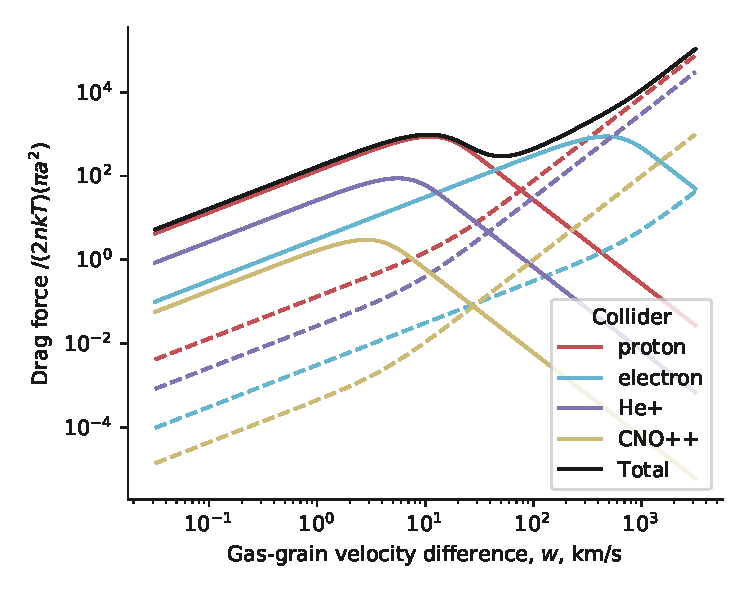
\includegraphics[width=\linewidth]{figs/test-Fdrag-components}
  \caption{Contributions of different collider species to the
    dimensionless drag force, \(f\drag / f_*\), as a function of
    gas--grain slip velocity, \(w\).  Solid lines show the Coulomb
    (electrostatic) drag, while dashed lines show the Epstein
    (solid-body) drag.  Results are shown for dimensionless grain
    potential \(\phi = 10\).  All Coulomb forces scale with
    \(\phi^2\), while the Epstein forces are independent of \(\phi\).  The
    species labelled ``CNO++'' represents the combined effect of all
    metals (see footnote~\ref{fn:metal-drag}).}
  \label{fig:drag-components}
\end{figure}


\begin{figure}
  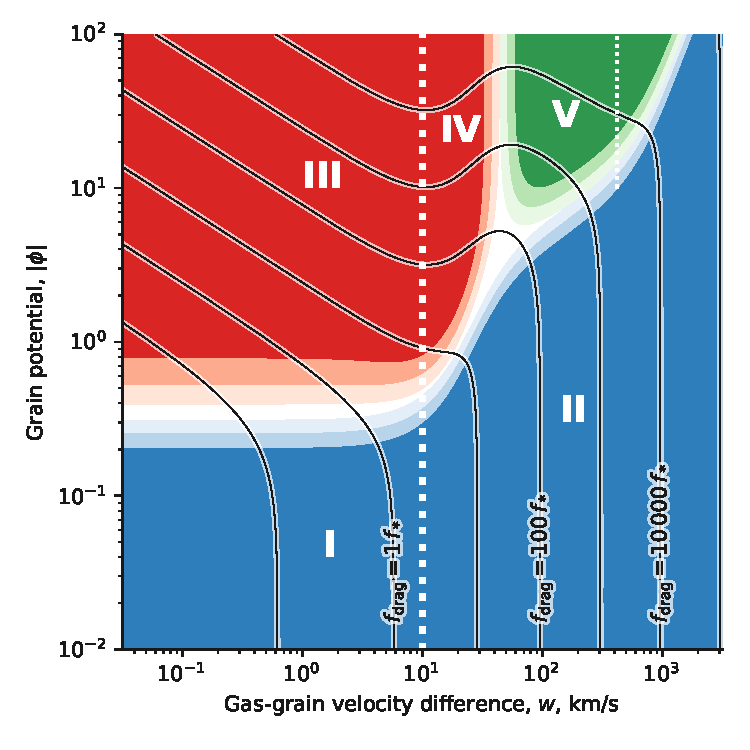
\includegraphics[width=\linewidth]{figs/test-Fdrag-param-space}
  \caption{Regimes of gas--grain drag as a function of slip velocity
    and grain potential.  The different regimes are indicated by bold
    roman numerals, as explained in
    Table~\ref{tab:fdrag-regimes}. Blue shading indicates regions
    dominated by Epstein (solid-body) drag, whereas red and green
    shading indicate regions dominated by Coulomb drag due to protons
    and electrons, respectively.  In each case, the saturated color
    represents a contribution \(> 70\%\) of the relevant component to
    the total drag force, while progressively lighter shading
    represents the \(> 60\%\) and \(> 50\%\) levels.  The thick white
    dotted line indicates the transition between the subthermal and
    superthermal regimes for protons, while the thin white dotted line
    indicates the corresponding transition for electrons.  Contours
    show the total drag force in units of \(f_*\) (see
    eq.~[\ref{eq:fstar}]) in decade intervals from \(0.1\) to
    \(10^4\), as labelled.  Results are shown for
    \(T = \SI{8000}{K}\) and \(n = \SI{100}{cm^{-3}}\), but the
    differences are very slight throughout the ranges
    \(T = \text{\SIrange{5000}{15000}{K}}\) and
    \(n = \text{\SIrange{e-3}{e6}{cm^{-3}}}\).}
  \label{fig:drag-v-phi-plane}
\end{figure}


\begin{figure*}
  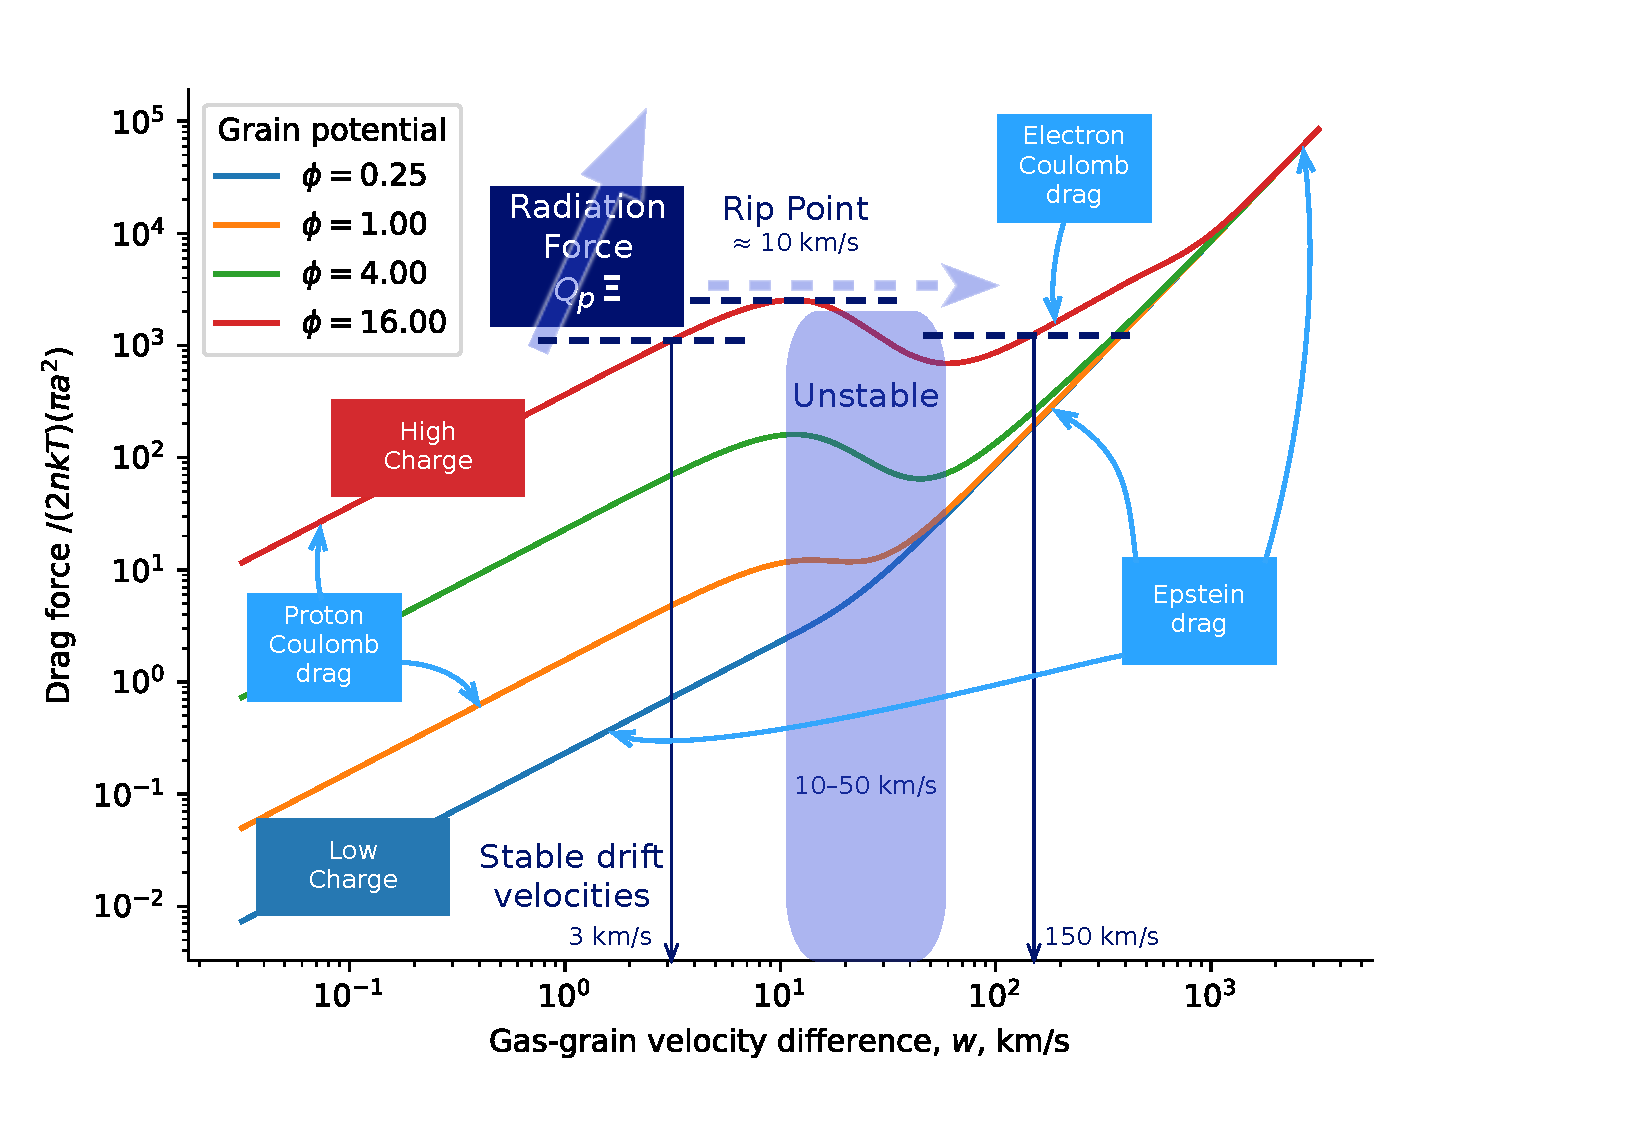
\includegraphics[width=\linewidth]{figs/gas-grain-drag-photoionized}
  \caption{Dimensionless drag force, \(f\drag / f_*\), as a function
    of gas--grain slip velocity, \(w\), for different values of the
    grain potential in thermal units, \(\phi\).  Contributions from
    proton and electron Coulomb (electrostatic) drag, as well as
    Epstein (solid-body) drag are indicated.  Examples of subsonic and
    highly supersonic stable drift velocities are shown (thin dark
    blue arrows), where the drag force is in equilibrium with the
    radiation force (thick dark blue dashed lines), while blue shading
    indicates the unstable, mildly supersonic velocity regime, where
    no stable drift equilibrium exists.  Inset graph shows \(\phi\) as a
    function of the radiation parameter,
    \(\Xi = P_{\mathrm{rad}} / P_{\mathrm{gas}}\) on a log--linear scale
    for a collection of Cloudy models (see
    Appendix~\ref{sec:cloudy-models-dust}).}
  \label{fig:gas-grain-drag-photoionized}
\end{figure*}


\begin{figure}
  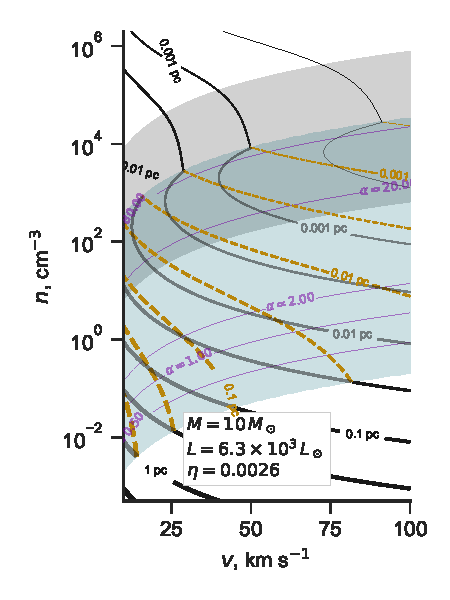
\includegraphics[width=\linewidth]{figs/decouple-v-n-plane}
  \caption{As Fig.~\ref{fig:zones-v-n-plane}(a), but accounting for
    gas-grain decoupling with constant efficiency \(\xi = 0.07\). }
  \label{fig:decouple-v-n-plane}
\end{figure}

\begin{figure}
  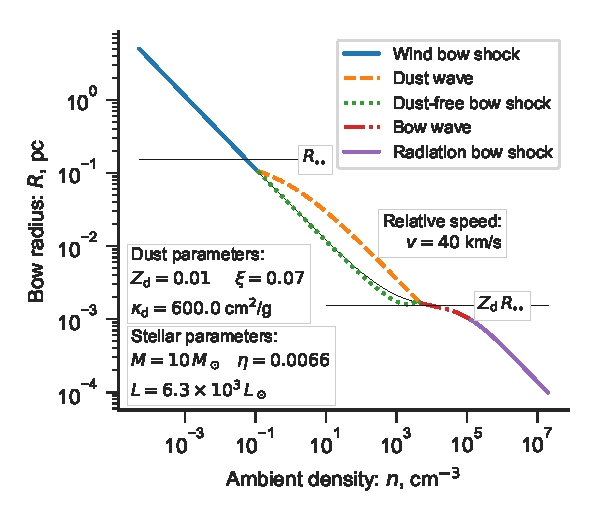
\includegraphics[width=\linewidth]{figs/decouple-v40-versus-n}
  \caption{Vertical cut through Fig.~\ref{fig:decouple-v-n-plane},
    showing bow radius and different regimes for a fixed inflow
    velocity of \SI{40}{km.s^{-1}}.}
  \label{fig:decouple-v40-versus-n}
\end{figure}


If the radiation field is sufficiently strong, then the collisional
coupling between grains and gas will break down.  In this section, we
calculate the regions of star+stream parameter space where this might
occur, leading to a separation of the bow into an outer dust wave and
an inner, dust-free bow shock.

\subsubsection{Drag force on grains}
\label{sec:drag-force-grains}

\begin{table}
  \centering
  \caption{Regimes of drag force as function of grain potential and slip speed}
  \label{tab:fdrag-regimes}
  \renewcommand\arraystretch{1.3}
  \resizebox{\linewidth}{!}{%
    \begin{tabular}{@{}r l l l@{}}
    \toprule
      & Regime & Approximate criteria & \(f\drag / f_*\) \\ \midrule
      I & Epstein subsonic & \(\phi^2 \ll 1\)
                             and \(w_{10} < 1\) & \(1.5\, w_{10}\) \\
      II & Epstein supersonic & \(w_{10} > 1\)
                                and \(w_{10} > 5\,\abs{\phi}\)& \( w_{10}^2\) \\
      III & Coulomb p\(^+\) subthermal & \(\phi^2 > 1\)
                                         and \(w_{10} < 1\) & \((1 + 20\, \phi^2)\,
                                                              w_{10}\) \\
    % & Coulomb p\(^+\) peak & \(\phi^2 > 1\)
    %                          and \(w_{10} \approx 1\) & \(1 + 10\, \phi^2\) \\
      IV & Coulomb p\(^+\) superthermal & \(\phi^2 > 1\)
                                          and \(1 < w_{10} < 5\) & \(w_{10}^2
                                                                   + 10\, \phi^2/w_{10}^2 \) \\
      V & Coulomb e\(^-\) subthermal & \(\phi^2 > 20\)
                                 and \(5 < w_{10} < 42\) & \(0.48\, \phi^2 \,
                                                           w_{10}\) \\
    \bottomrule
  \end{tabular}
  }
\end{table}

The drag force on a charged dust grain moving at a relative speed
\(w\) through a plasma has contributions from both direct collisions
and from electrostatic Coulomb interactions with ions and electrons.
We use the expressions in \citet{Draine:1979a}, equations~(4)--(6),
considering the contributions from protons, electrons, helium
ions,\footnote{Helium is assumed to be singly ionized, leading to only
  a small contribution to the drag force.  For much hotter stars, such
  as the central stars of planetary nebulae, helium may be doubly
  ionized, which leads to a fourfold increase in its Coulomb drag
  contribution, which is significant for \(w < \SI{5}{km.s^{-1}}\).} %
and metal ions.\footnote{%
  \label{fn:metal-drag}
  All metals are lumped together as a single species, assuming
  standard \hii{} region gas-phase abundances.  They are dominated by
  C and O, with minor contributions from N and Ne.  The total
  abundance is \num{8.5e-4} and the effective atomic weight is
  \num{15.3}.  All are assumed to be doubly ionized.  Their largest
  relative contribution to the drag force is for
  \(w < \SI{2}{km.s^{-1}}\), but is less than 1\% even there.} %
Results are shown in Figure~\ref{fig:drag-components}, where dashed lines correspond to direct solid body collisions and solid lines to electrostatic interactions.  The latter depend on the grain potential, which is described in dimensionless terms by \(\phi\), which is the electrostatic potential
energy of a unit charge at the surface of a grain of charge
\(z\grain\) and radius \(a\), in units of the characteristic thermal
energy of a gas particle:
\begin{equation}
  \label{eq:phi-potential}
  \phi = \frac{e^2 z\grain}{a kT} \ .
\end{equation}
The electrostatic contributions to \(f\drag\) are proportional to
\(\phi^2\) (results are shown for \(\abs{\phi} = 10\)), whereas the
solid-body contributions are independent of \(\phi\).  The drag force is
put in dimensionless units by dividing by a characteristic force:
\begin{equation}
  \label{eq:fstar}
  f_* = 2 n k T \cdot \pi a^2 \ , 
\end{equation}
which is approximately\footnote{%
  To simplify the exposition, the gas pressure in this section is
  calculated assuming a fully ionized, pure hydrogen plasma, yielding
  \(P\gas = 2 n k T\). For typical ISM abundances, the contribution of
  helium and its corresponding electrons yield a correction to this of
  order 5\%.  The required modifications when a cool star interacts
  with a predominantly neutral gas stream are discussed later.  } %
the ionized gas pressure multiplied by the grain geometric cross
section.

For grains with low electric charge, \(\phi^2 \ll 1\), the drag force is
dominated by direct collisions of protons with the grain (dashed red
line in Fig.~\ref{fig:drag-components}).  The gas collisional mean
free path is much larger than the grain size, so the drag is in the
Epstein regime \citep{Weidenschilling:1977b}.
% This is illustrated by
% the \(\phi = 0.25\) case (blue line) in
% Figure~\ref{fig:gas-grain-drag-photoionized}.
As the relative gas--grain slip speed, \(w\), increases, \(f\drag\)
first increases linearly with \(w\) reaching \(f\drag \approx f_*\) at
\(w = \sound \approx \SI{10}{km.s^{-1}}\), then transitions to a quadratic
increase in the supersonic regime.

As \(\abs{\phi}\) increases, long-range electrostatic interactions with
protons within the Debye radius (Coulomb drag) become increasingly
important at subsonic relative velocities, as shown by the solid lines
in Figure~\ref{fig:drag-components}).
% in
% Figure~\ref{fig:gas-grain-drag-photoionized} by the orange
% (\(\phi = 1\)), green (\(\phi = 4\)), and red (\(\phi = 16\)) lines.
However, the Coulomb drag has a peak when \(w\) is equal to the
thermal speed of the colliders, which is
\(\approx \SI{10}{km.s^{-1}}\) for protons, giving a maximum strength of
\begin{equation}
  \label{eq:fdrag-maximum}
  f_{\mathrm{max}} = 0.5\, (\ln\Lambda)\, \phi^2 f_* \approx 10\, \phi^2 f_* \ , 
\end{equation}
where \(\Lambda\) is the plasma parameter (number of particles within a
Debye volume), such that
\(\ln\Lambda = 23.267 + 1.5 \ln T_4 - 0.5 \ln n\).  At highly super-thermal
speeds, the Coulomb drag falls asymptotically as
\(f\drag \propto 1 / w^{2}\).  The thermal speed of electrons is higher than
that of the protons by a factor of \((m_p / m_e)^{1/2}\), so that the
electron Coulomb drag (solid light blue line) gives a second peak of
similar strength, but at \(w \approx \SI{430}{km.s^{-1}}\).  The behavior of
\(f\drag\) in all these different regimes is summarised in
Table~\ref{tab:fdrag-regimes}, in terms of \(\phi\) and
\(w_{10} = w / \SI{10}{km.s^{-1}}\).  This is further illustrated in
Figure~\ref{fig:drag-v-phi-plane}, where each of the drag regimes is
located on the \((w, \abs{\phi})\) plane.


% \begin{equation}
%   \label{eq:fdrag-regimes}
%   f\drag \approx
%   \begin{cases}
%     \text{Epstein subsonic (\(\phi^2 \ll 1\) and \(w_{10} < 1\)):}
%     & w_{10}\, f_* \\
%     \text{Epstein supersonic (\(\phi^2 \ll 1\) and \(w_{10} > 1\)):}
%     & w_{10}^2\, f_* \\
%     \text{Coulomb p\(^+\) subthermal (\(\phi^2 > 1\) and \(w_{10} < 1\)):}
%     & (1 + 20 \phi^2)\, w_{10}\, f_* \\
%     \text{Coulomb p\(^+\) peak (\(\phi^2 > 1\) and \(w_{10} \approx 1\)):}
%     & (1 + 10 \phi^2)\, f_* \\
%     \text{Coulomb p\(^+\) superthermal (\(\phi^2 > 1\) and \(1 < w_{10} < 5\)):}
%     & (w_{10}^2 + 10 \phi^2/w_{10}^2) \, f_* \\
%     \text{Coulomb e\(^-\) subthermal (\(\phi^2 > 20\) and \(5 < w_{10} < 42\)):}
%     & 0.48 \phi^2 \, w_{10}\, f_* \\
%   \end{cases}
% \end{equation}

% Or \Lambda = (4 pi / 3) n r_D^3?
% Where Debye length is r_D^2 = k T / 4 pi n e^2
% => \Lambda = n r_D (4 pi / 3) k T / 4 pi n e^2
% = k T r_D / 3 e^2
% This is 9 times less than the other expression
% Anyway, from kappa notes I have
% \ln\Lambda = 9.452 + 1.5 ln(T) - 0.5 ln(n)

% If I am going to use log10, then the coefficients get divided by
% ln(10) = 2.30258509299, and if we use T4, then we add 1.5 ln(1e4) =
% 13.815.  So we get 23.267 + 0.651 log10(T4) - 0.217 log10(n).  Nope,
% best with natural log

\subsubsection{Gas--grain separation: drift and rip}
\label{sec:gas-grain-separ}

In Appendix~\ref{sec:gas-free-bow} we calculate the behaviour of an
incoming stream of dust grains, subject only to the repulsive
radiation force from a star.  For an initial inward radial trajectory,
the dust grain motion is decelerated and turned around, reaching a
minimum radius \(R\starstar\), given by equation~\eqref{eq:dust-r0}.
This drag-free radiative turnaround radius, \(R\starstar\), is smaller
for higher initial inward velocities, but is independent of the
density of the incoming stream.  We are now in a position to see how
gas--grain drag will modify this picture.

From equations~\eqref{eq:dust-rad-force} and~\eqref{eq:fstar}, we can
write the radiation force acting on a grain as
\begin{equation}
  \label{eq:frad-Xi}
  f\rad = \Qp\, \Xi\, f_* \ ,
\end{equation}
where \(\Qp\) is the grain's radiation pressure efficiency (see
footnote~\ref{fn:Qp} in Appendix~\ref{sec:gas-free-bow}) and \(\Xi\) is
the local radiation parameter, defined as the ratio of direct stellar
radiation pressure to gas pressure:
\begin{equation}
  \label{eq:Xi-Prad-over-Pgas}
  \Xi \equiv \frac{P\rad}{P\gas} \approx \frac{L}{4 \pi R^2 c\, (2 n k T)} \ ,
\end{equation}
where the last expression corresponds to the optically thin limit.
The grain potential \(\phi\) is also primarily determined by \(\Xi\), as
shown in Appendix~\ref{sec:cloudy-models-dust} and the inset graph of
Figure~\ref{fig:gas-grain-drag-photoionized}, but with a slow
dependence, which can be approximated as
\begin{equation}
  \label{eq:phi-vs-Xi}
  \phi(\Xi) \approx 1.5 \bigl( 2.3 +  \ln \Xi \bigr) \ .
\end{equation}
There are also slight secondary dependencies on the grain composition and
stellar spectrum.  The relationship given in eq.~\eqref{eq:phi-vs-Xi}
is appropriate for graphite grains and for stellar effective
temperatures in the range \SIrange{20}{30}{kK}.  For hotter stars than
this, \(\phi\) should be multiplied by a further factor of \(1.5\), while
for silicate grains it should be divided by \(1.5\).

In the outer regions of the photoionized volume around an OB star,
close to the ionization front, the radiation parameter is low, with
typical value \(\Xi \sim 0.1\).  In this regime, the negative charge
current at the grain surface due to electron collisions is roughly in
balance with the positive current due to the ultraviolet photoelectric
effect \citep{Weingartner:2001b}, leading to a low grain potential,
\(\abs{\phi} < 1\), which may be positive or negative.  The low
\(\Xi\) means that the radiative force is also weak:
\(f\rad \sim 0.1 f_*\) from equation~\eqref{eq:frad-Xi} if
\(\Qp \sim 1\) at UV wavelengths, which is true for all but the smallest
grains.  Thus, from the equations for \(f\drag\) given in
Table~\ref{tab:fdrag-regimes}, the radiative force can be balanced by
Epstein drag if \(w_{10} \sim 0.1\), leading to a small equilibrium drift
velocity, \(w\drift < \SI{1}{km.s^{-1}}\), of the grains with respect
to the gas.  This drift is much smaller than the inward stream
velocities that we are considering
(\(v_\infty > \SI{10}{km.s^{-1}}\)), so the dust follows the gas stream at
a slightly reduced velocity (\(< 10\%\)), and (by mass conservation) a
slightly increased density.  Each grain exerts an exactly opposite
force to \(f\drag\) upon the gas, but since the dust-gas mass ratio,
\(Z\grain\), is small, this produces a negligible acceleration of the
gas.

\begin{table}
  \caption{Critical values of radiation parameter at the rip point: \(\Xi_\dag\)}
  \centering
  \begin{tabular*}{0.75\columnwidth}{l @{\quad\quad\quad\quad} S S} \toprule
    & \multicolumn{2}{c}{Grain composition} \\
    Spectrum & {Graphite} & {Silicate}
    \\ \midrule
    B star & 1000 +- 400 & 350 +- 150 \\
    O star & 3000 +- 500 & 2500 +- 500 \\
    \bottomrule
    \addlinespace
    \multicolumn{3}{@{}p{0.75\columnwidth}@{}}{
    Calculated from the Cloudy models shown in Figure~\ref{fig:drift-gn}. 
    Uncertainties represent variations with grain size and gas density. 
    See Appendix~\ref{sec:cloudy-models-dust} for further details.}
  \end{tabular*}
  \label{tab:Xi-rip}
\end{table}

As the dusty stream approaches the star, the radiation parameter
\(\Xi\) will increase, with a dependence of \(R^{-2}\) once the stream
is well inside the ionization front.  This increases \(f\rad\)
(eq.~[\ref{eq:frad-Xi}]), but also increases the grain potential,
\(\phi\) (eq.~[\ref{eq:phi-vs-Xi}]) due to the increasing dominance of
grain charging by photoelectric ejection.  Initially, this results in
a lowering of the equilibrium drift velocity to \(w_{10} \sim 0.01\) as
the Coulomb drag kicks in (see Appendix~\ref{sec:cloudy-models-dust}).
However, at smaller radii the slow logarithmic increase in
\(\phi(\Xi)\) means that the drift velocity must start increasing again to
accommodate the linear increase of \(f\rad(\Xi)\).  Eventually,
\(f\rad\) exceeds \(f_{\mathrm{max}}\), the maximum drag force that
proton Coulomb interactions can provide
(eq.~[\ref{eq:fdrag-maximum}]).  This occurs at a critical value of
the radiation parameter, which we denote the \textit{rip point}:
\(\Xi_\dag \sim 1000\).  The variations in \(\Xi_\dag\) with star and grain
parameters, which are of order \SI{+- 0.5}{dex}, are listed in
Table~\ref{tab:Xi-rip} and illustrated graphically in
Figure~\ref{fig:drift-gn}.

\subsubsection{Existence conditions for dust waves}
\label{sec:exist-cond-separ}

In order for a separate dust wave to exist, it is necessary for the
grains to decouple from the incoming gas stream before the stream hits
the hydrodynamic bow shock caused by the stellar wind.  The radius of
the rip point, \(R_\dag\), can be expressed in terms of \(R_*\), the
fiducial optically thick bow shock radius introduced in
\S~\ref{sec:strong-gas-grain}:
\begin{equation}
  \label{eq:Rdag-over-Rstar}
  R_\dag = \frac{v_\infty}{\sound}\, \Xi_\dag^{-1/2} R_* \approx v_{10}\, \Xi_\dag^{-1/2} R_* \ ,
\end{equation}
where we have made use of equations~\eqref{eq:Rstar}
and~\eqref{eq:Xi-Prad-over-Pgas}.  The wind bow shock radius is
\(R_0 = \eta^{1/2} R_*\) (eq.~[\ref{eq:x-cases}]), where \(\eta\) is the
wind momentum efficiency (eq.~[\ref{eq:wind-eta-typical}]).
Therefore, the condition \(R_\dag > R_0\) becomes
\begin{equation}
  \label{eq:dust-wave-velocity-condition}
  v_{10} > v_{10,\text{min}} = \bigl( \Xi_\dag \, \eta \bigr)^{1/2} \ . 
\end{equation}
For O stars, the wind efficiency is generally high (\(\eta > 0.1\)) and
\(\Xi_\dag > 2000\) (Tab.~\ref{tab:Xi-rip}), so that dust waves can only
exist when the stream velocity is very high
(\(v_\infty > \SI{150}{km.s^{-1}}\)).  For B~stars, in contrast, the wind
can be much weaker (\(\eta < 0.01\)) and \(\Xi_\dag\) is also smaller, so
that dust waves are permitted by this criterion for much lower stream
velocities: (\(v_\infty > \SI{30}{km.s^{-1}}\)).

\begin{figure*}
  \centering
  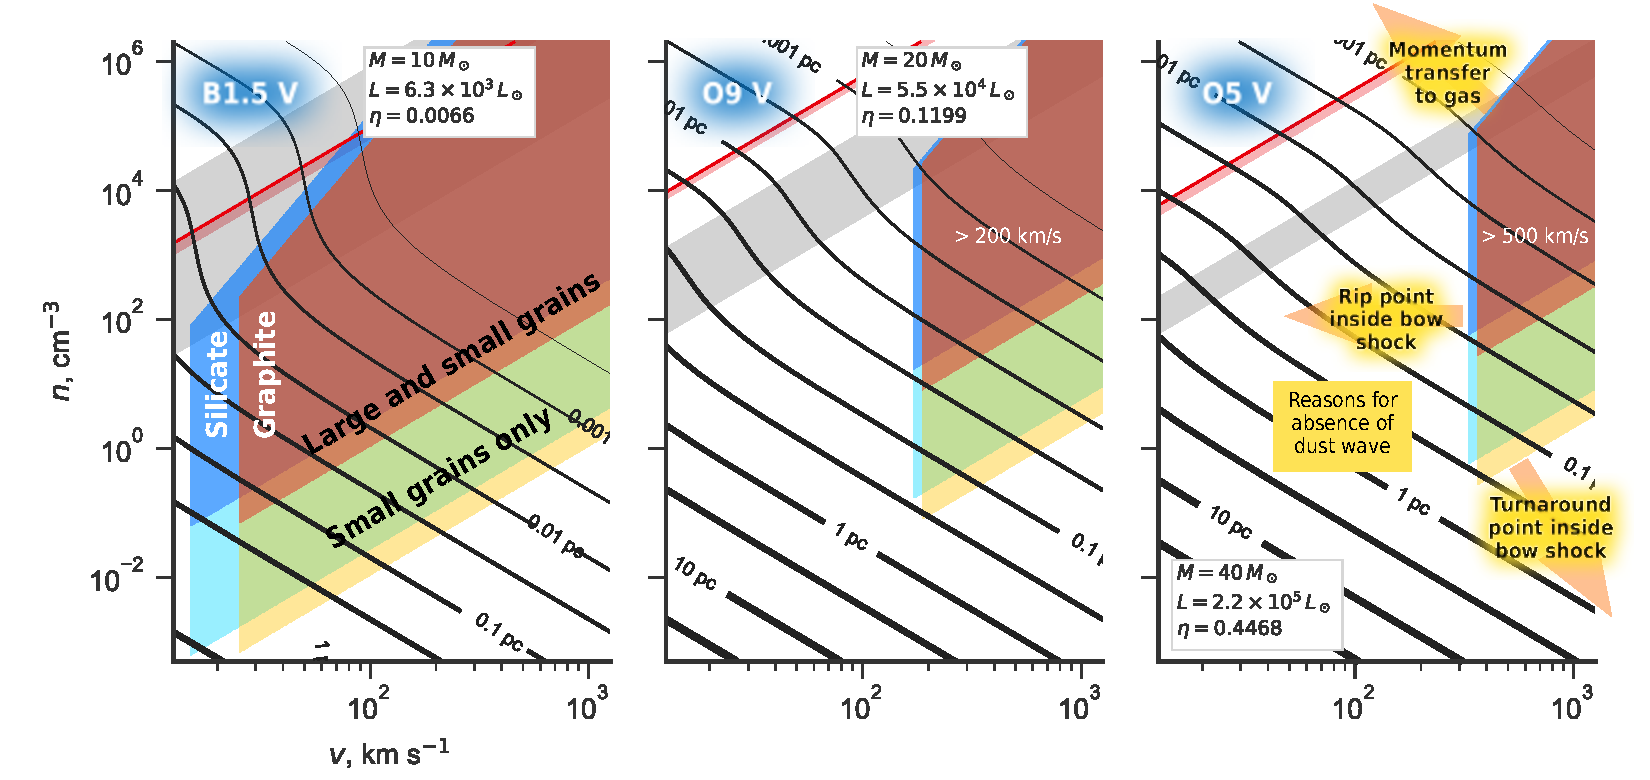
\includegraphics[width=\linewidth]{figs/existence-dust-wave}
  \caption{Regions of stream parameter space \((v, n)\) where dust
    waves may form around main-sequence OB stars of
    \SIlist{10;20;40}{M_\odot} (see Tab.~\ref{tab:stars}).  Figure is
    similar to Fig.~\ref{fig:zones-v-n-plane}, except that the
    velocity axis is logarithmic and extends out to
    \SI{1000}{km.s^{-1}}.  Overlapping colored shapes show parameters
    where dust waves may be allowed in the cases of large
    (\(a = \SI{0.2}{\um}\)) and small (\(a = \SI{0.02}{\um}\))
    graphite and silicate grains, as labeled in the left panel.  For
    \((v, n)\) outside of these shapes, dust waves cannot occur for
    the reasons indicated by labeled orange arrows in the center
    panel.  Labeled dashed lines in the right panel show the
    correspondence between the region boundaries and each dust wave
    existence condition given in
    equations~(\ref{eq:dust-wave-velocity-condition},
    \ref{eq:dust-wave-low-density-condition},
    \ref{eq:dust-wave-high-density-condition}). Heavy dashed lines in
    the left panel show where the rip point and the drag-free
    turnaround radius coincide.  For dust waves below these lines,
    drag forces are unimportant for the grains.  }
  \label{fig:existence-dust-wave}
\end{figure*}

However, there are other conditions that need to be satisfied in order
for the dust wave to exist.  For instance, the drag-free turnaround
radius must also be outside the bow shock: \(R\starstar > R_0\),
otherwise the radiation is incapable of repelling the grain
opportunely, even once it has decoupled from the gas.  From
equations~\eqref{eq:Rstar}, \eqref{eq:tau-star},
and~\eqref{eq:dust-r0} we find
\begin{equation}
  \label{eq:Rstarstar-over-Rstar}
  \frac{R\starstar}{R_*} = \frac{2 \sigma\grain \Qp \tau_*}{\kappa m\grain} \ , 
\end{equation}
so, if we define a single-grain opacity as
\(\kappa\grain = \sigma\grain \Qp / m\grain\), then this condition becomes
\begin{equation}
  \label{eq:dust-wave-low-density-condition}
  \tau_* >  \tau_{*,\text{min}} = 0.5\, \frac{\kappa}{\kappa\grain}\, \eta^{1/2} 
  % \frac{\kappa \eta^{1/2}}{2 \kappa\grain}
  \ . 
\end{equation}
The average value of the factor \(\kappa / \kappa\grain\) over the entire grain
population must be equal to the dust--gas mass ratio,
\(Z\grain \approx 0.01\), but the factor will vary between grains, according
to their size and composition.\footnote{%
  Remember that \(\kappa\) is the opacity per unit mass of gas, while
  \(\kappa\grain\) is the opacity per unit mass of a particular grain. In
  both cases, averaged over the stellar spectrum.} %
In particular, it will be relatively larger for the largest grains
(\(a \approx \SI{0.2}{\um}\)), which dominate the total dust mass, and
smaller for the smaller grains (\(a \approx \SI{0.02}{\um}\)), which
dominate the UV opacity.  Given the dependence of \(\tau_*\) on the
stream parameters (eq.~[\ref{eq:taustar-typical}]), for a given
stellar luminosity this condition corresponds to a minimum value for
\(n / v_\infty^2\).

A third condition comes from requiring \(R_\dag > R_0\) in the radiation
bow wave regime (see \S~\ref{sec:three-bow-regimes}), where
\(R_0 \approx 2 \tau_* R_*\).  This yields
\begin{equation}
  \label{eq:dust-wave-high-density-condition}
  \tau_* < \tau_{*,\text{max}} = 0.5\, v_{10}\, \Xi_\dag^{-1/2} \ , 
\end{equation}
which, for a given stellar luminosity, corresponds to a maximum value
for \(n / v_\infty^4\).  Thus, for a given stream velocity that satisfies
equation~\eqref{eq:dust-wave-velocity-condition},
equations~(\ref{eq:dust-wave-low-density-condition},
\ref{eq:dust-wave-high-density-condition}) determine respectively the
minimum and maximum stream density for which a dust wave can exist.

Further restrictions on the existence of dust waves arise when the
effects of magnetic fields are considered, as will be discussed in
\S~\ref{sec:magn-effects-grain} below.

\subsubsection{Grain trajectories along the symmetry axis}
\label{sec:grain-traj-along}

What happens to the dust grain following this catastrophic breakdown
of gas--grain coupling depends on the relation between the rip point
radius, \(R_\dag\), and the drag-free radiative turnaround radius,
\(R\starstar\).  If \(R_\dag > R\starstar\), then the grain's inertia
will still carry it in as far as \(R\starstar\) and the initial
trajectory will be almost identical to that described in
Appendix~\ref{sec:gas-free-bow} for the drag-free case. However, after
being turned around by the radiation field and pushed out past
\(R_\dag\) again, the grain will \emph{recouple} to the gas and be
dragged back for a second approach.\footnote{If the initial impact
  parameter of the trajectory is not strictly \(b = 0\), then the
  resultant lateral component of \(f\rad\) will mean that \(b\) will
  be much increased for the second approach.} %
From equations~(\ref{eq:Rdag-over-Rstar},
\ref{eq:Rstarstar-over-Rstar},
\ref{eq:dust-wave-high-density-condition}), the condition
\(R_\dag > R\starstar\) corresponds to
\(\tau_* < (\kappa/\kappa\grain) \tau_{*,\text{max}}\), which is indicated by dashed
lines in the left panel of Figure~\ref{fig:existence-dust-wave}.  If,
on the other hand, \(R_\dag < R\starstar\), then the tail wind provided
by the gas carries the grain closer to the star than its inertia would
naturally take it.  When the grain finally decouples at \(R_\dag\) it
experiences a much higher unbalanced \(f\rad\), which can initially
accelerate it to outward velocities significantly higher than the
inflow velocity if \(R_\dag \ll R\starstar\).

\begin{figure*}
  \centering
  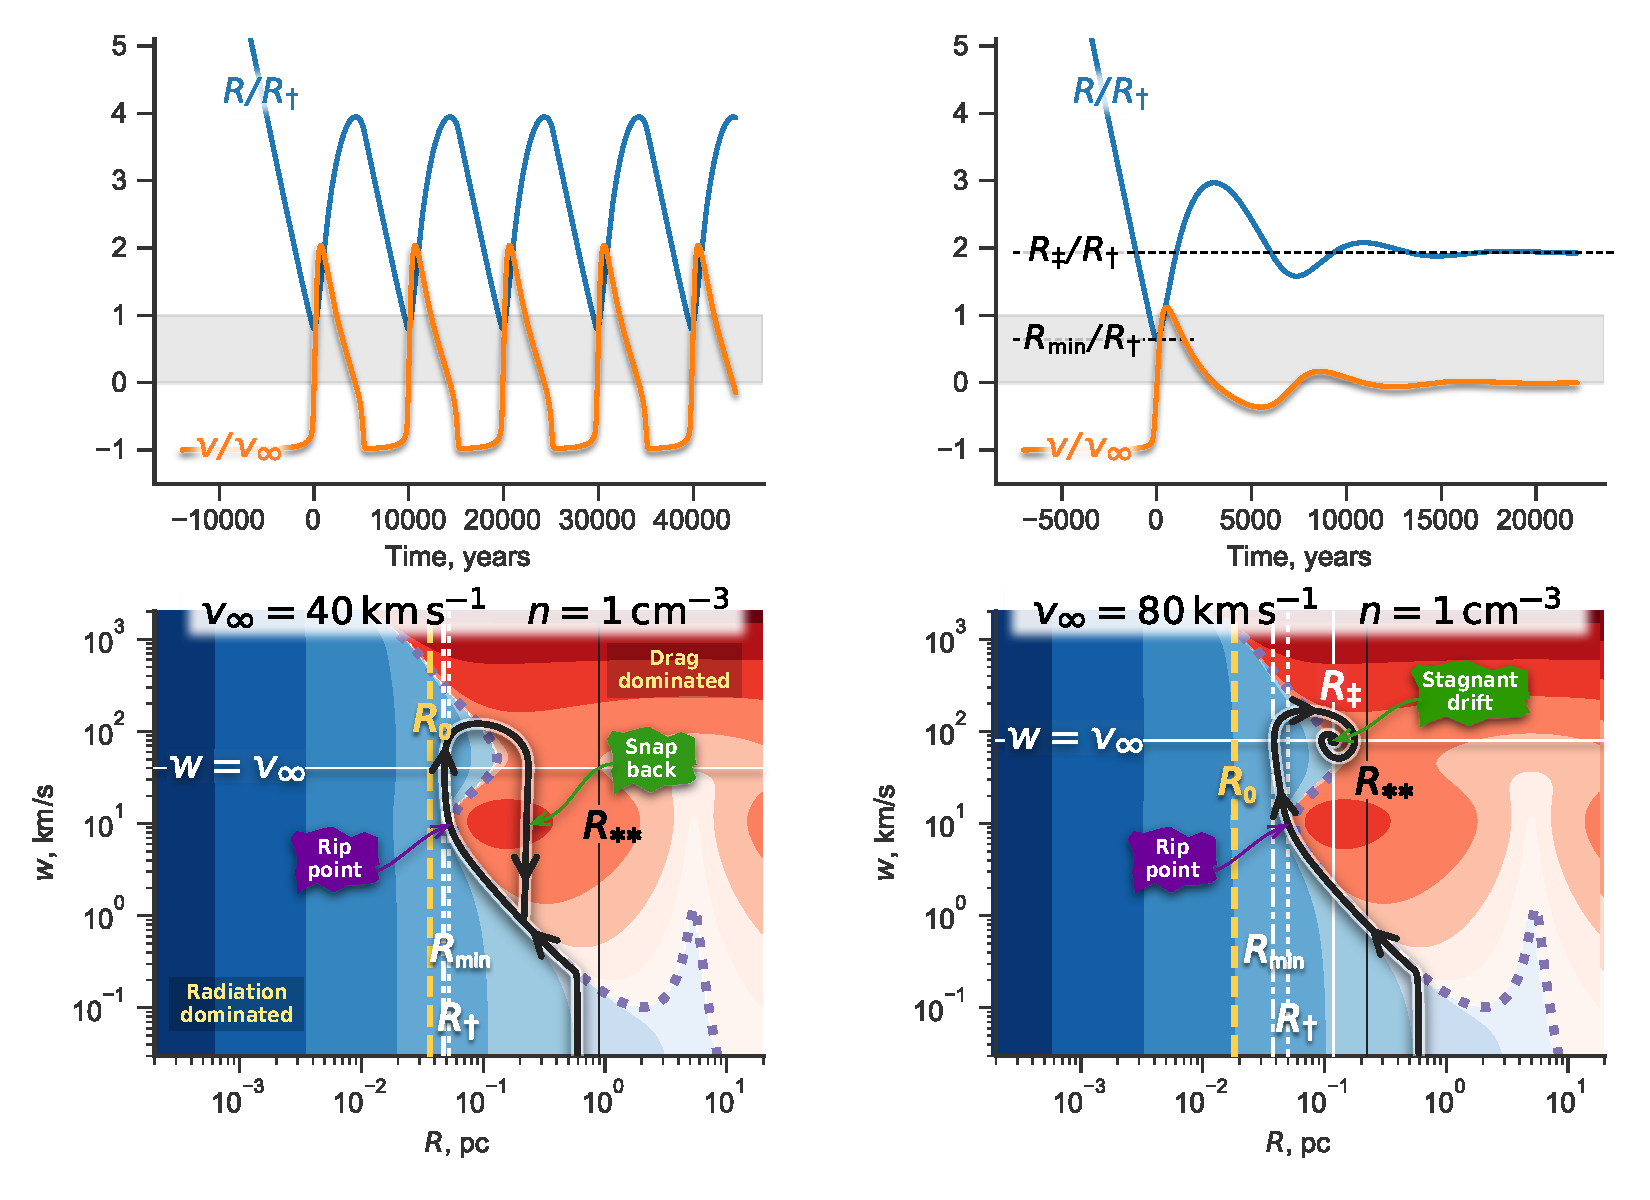
\includegraphics[width=\linewidth]{figs/dust-wave-phase-trajectories-annotate}
  \caption{Trajectories of small graphite grains
    (\(a = \SI{0.02}{\um}\)) at impact parameter \(b = 0\) for two
    example cases (see yellow ``+'' symbols in left panel of
    Fig.~\ref{fig:existence-dust-wave}), which differ only in the
    stream velocity: \(v = \SI{40}{km.s^{-1}}\) (left panels) and
    \SI{80}{km.s^{-1}} (right panels).  In both cases, the stream
    density is \(n = \SI{1}{cm^{-3}}\) and the central star is a
    \SI{10}{M_\odot} main-sequence B star (see Tab.~\ref{tab:stars}).
    Upper panels show the evolution of grain radius, \(R\) (blue
    curve, normalized by the rip point radius, \(R_\dag\)), and grain
    velocity, \(v\) (orange curve, normalized by the gas stream
    velocity).  The origin of the time axis is set to the moment of
    closest approach of the grain to the star: \(R = \Rmin\).  Lower
    panels show the trajectories in phase space: position versus
    gas--grain relative slip velocity (\(w = \abs{v - v_\infty}\)).  Filled
    contours show the net force on the grain: \(f\rad - f\drag\), with
    positive values in blue and negative values in red.  The heavy
    dotted line shows where there is no net force: \(f\rad = f\drag\).
    The grain trajectory (thick, solid black line with arrows)
    initially follows this line, but departs from it after the rip
    point. In the left panel, the grain enters a limit cycle between
    decoupling (rip) and re-coupling (snap back).  In the right panel,
    the grain spirals in on the stagnant drift point.  See text for
    further details.}
    \label{fig:phase-space-trajectories}
\end{figure*}

The post-decoupling behavior of the grain depends on the sign of
\(d f\drag / d w\) when \(w = \abs{v_\infty}\).  If this derivative is
positive, as is the case in drag regimes~II and V (see
Tab.~\ref{tab:fdrag-regimes} and Fig.~\ref{fig:drag-v-phi-plane}),
then the grain can reach a stable equilibrium drift at rest with
respect to the star\footnote{%
  Again, this is only strictly true when the impact parameter is zero.
  However, as we show below, it is a reasonable approximation over a
  range of impact parameters in the case where the angle between the
  magnetic field direction and the stream velocity is not too
  large.} %
at a point \(R_\ddag\), which we call the \textit{stagnant drift
  radius}. If the stream velocity is not excessively high
(\(v_\infty < \SI{150}{km.s^{-1}}\) when \(\phi = 4\), or
\(< \SI{300}{km.s^{-1}}\) when \(\phi = 16\)), then the equilibrium
\(f\rad\) is less than the value at the rip point, requiring a lower
value of the radiation parameter: \(\Xi_\ddag < \Xi_\dag\).  The resultant
stagnant drift radius is therefore outside the rip point:
\(R_\ddag > R_\dag\).

On the other hand, if \(d f\drag / d w < 0\) when
\(w = \abs{v_\infty}\), then the equilibrium is unstable and no stagnant
drift is possible.  This occurs for drag regime~IV, which applies when
\(\phi > 1\) and
\(\SI{10}{km.s^{-1}} < v_\infty < \SI{50}{km.s^{-1}}\).  There is also a
second unstable regime (partially visible in the upper-right corner of
Fig.~\ref{fig:drag-v-phi-plane}), which is related to the thermal peak
in the electron Coulomb drag when \(\phi > 30\) and
\(\SI{400}{km.s^{-1}} < v_\infty < \SI{2000}{km.s^{-1}}\), but this is not
relevant to bow shocks around OB~stars.\footnote{%
  It may apply in other contexts, such as outflows from AGN, since
  detailed modeling of grain charging around quasars
  \citep{Weingartner:2006a} implies that grain potentials as high as
  \(\phi \sim 100\) can be achieved.} %

An examples of each of these two behaviors is illustrated in
Figure~\ref{fig:phase-space-trajectories}.  The left panels show the
case where \(v_\infty = \SI{40}{km.s^{-1}}\), which is in the unstable
regime, resulting in periodic ``limit-cycle'' behavior (the parameters
of this model correspond to the yellow ``plus'' symbol labeled ``40''
in the left panel of Fig.~\ref{fig:existence-dust-wave}).  During the
grain's first approach, it starts to follow a phase trajectory (lower
left panel) along the \(f\rad - f\drag = 0\) contour, corresponding to
equilibrium drift, in which the grain begins to move a few
\si{km.s^{-1}} slower than the gas stream.  Then, when it reaches the
rip point (\(R = R_\dag\), \(w \approx \SI{10}{km.s^{-1}}\)) it suddenly
experiences a large unbalanced outward radiation force (blue region of
phase space in Fig.~\ref{fig:phase-space-trajectories}). The grain's
inward momentum carries it to the point \(\Rmin \approx 0.85 R_\dag\), before
it is expelled at roughly twice the inflow speed.  However, after
moving outward, it finds itself in a drag-dominated region of phase
space (red in the figure), and so recouples to the inflowing gas
stream.  The recoupling initiates gradually, as the grain's outward
motion is slowed and it begins to move inward again, but is completed
suddenly once \(w\) again falls below \SI{10}{km.s^{-1}}, in what we
term \textit{snap back}. The net result is that the grain has returned
to exactly the same phase track that it started in on, and so repeats
the cycle indefinitely.

The right panels of Figure~\ref{fig:phase-space-trajectories} show the
case where the stream velocity is doubled to
\(v_\infty = \SI{80}{km.s^{-1}}\), but all other parameters remain the
same.  At this velocity, the equilibrium drift is stable and so the
grain can achieve a stagnant drift solution, where it is stationary
with respect to the star.  The trajectory during the first approach is
similar to the previous case, except that the overshoot of the rip
point is greater, so that \(\Rmin \approx 0.65 R_\dag\) in this case.  This is
a consequence of the fact that the rip point is closer to the
drag-free turnaround radius (\(R_\dag / R\star\star\) is not so small as in the
lower velocity case), so that the grain inertia is relatively more
important.  A second consequence is that the speed of the initial
expulsion is not so large, being only a little higher than the inflow
velocity (but opposite to it).  The qualitative difference between the
two cases emerges after the first recoupling: instead of the snap back
and endless limit cycle, the grain oscillates about the stagnant drift
radius with ever decreasing amplitude, so that it has come almost to
rest after a few oscillation periods.


\subsubsection{Magnetic effects on grain trajectories }
\label{sec:magn-effects-grain}



\section{The case of inside-out bows}
\label{sec:case-inside-out}

So far, we have considered the case where the inner source dominates
the radiation, while dust is present only in the outer stream, which
applies to hot stars interacting with the ISM.  However, in the case
of cool stars, the inner wind will also be dusty.  Examples are the
red supergiant (RSG) phase of high-mass evolution, or the asymptotic
giant branch (AGB) stage of low/intermediate-mass evolution.  In both
these cases, it is still the inner source that provides the radiation
field.  However, not all winds are radiatively driven and in those
cases it is conceivable that it is the outer source that dominates the
radiation field.  An example is the case of photoevaporating
protoplanetary disks (proplyds) in the Orion Nebula and other \hii{}
regions \citep{ODell:1994a}.  In the proplyds, the inner wind is a
thermally driven photoevaporation flow \citep{HA:1998, Henney:1999a},
while the outer stream is the stellar wind from an O~star
\citep{Garcia-Arredondo:2001a}.


%%% Local Variables:
%%% mode: latex
%%% TeX-master: "dusty-bow-wave"
%%% End:

\section{A simple model for stellar bows}
\label{sec:strong-gas-grain}

\begin{figure*}
  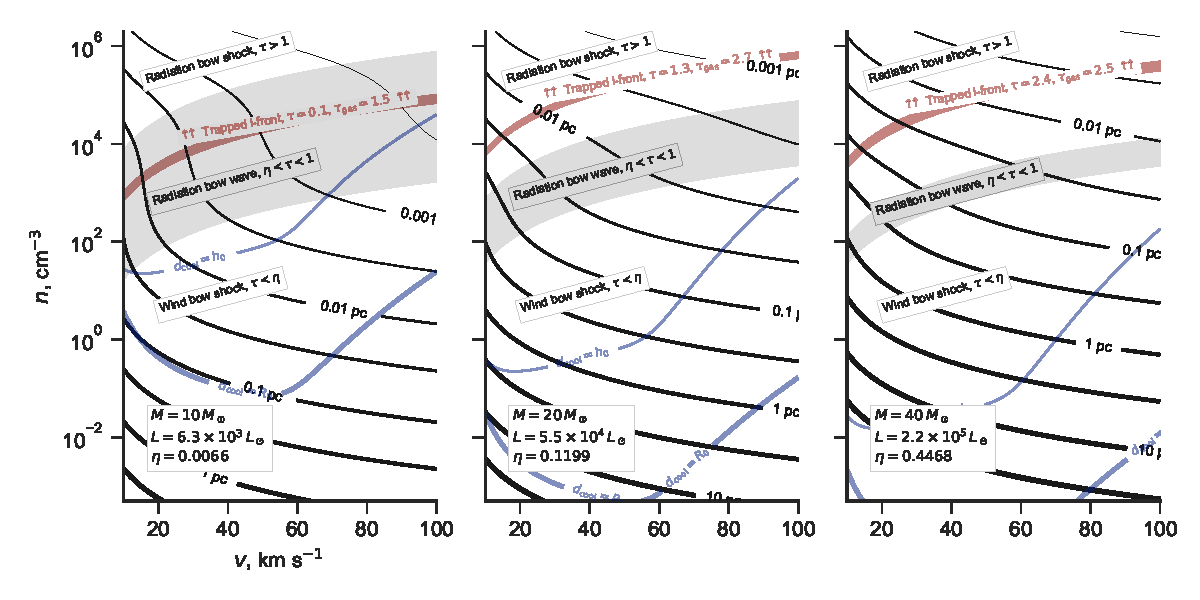
\includegraphics[width=\linewidth]{figs/zones-v-n-plane}
  \caption{Bow regimes in parameter space (\(v, n\)) of the external
    stream for main-sequence OB stars of different masses:
    (a)~\SI{10}{M_\odot}, (b)~\SI{20}{M_\odot}, (c)~\SI{40}{M_\odot}.  In all
    cases, \(\kappa = \SI{600}{cm^2.g^{-1}}\) and efficient gas-grain
    coupling is assumed. Solid black lines of varying thickness show the
    bow size (star-apex separation, \(R_0\)), while gray shading shows
    the radiation bow wave regime, with lower border
    \(\tau = \eta\wind\) and upper border \(\tau = 1\), where
    \(\tau = 2 \kappa \rho R_0\) is the optical depth through the bow.  For bows
    above the red solid line, the ionization front is trapped inside
    the bow (\S~\ref{sec:trapp-ioniz-front}).  Blue lines delineate
    different cooling regimes (\S~\ref{sec:radi-cool-lengths}).  Above
    the thin blue line (\(d_{\text{cool}} = h_0\)), the bow shock
    radiates efficiently, forming a thin shocked shell.  Below the
    thick blue line (\(d_{\text{cool}} = R_0\)), the bow shock is
    essentially non-radiative.}
  \label{fig:zones-v-n-plane}
\end{figure*}


We consider the canonical case of a bow around a star of bolometric
luminosity, \(L\), with a radiatively driven wind, which is immersed
in an external stream of gas and dust with density, \(\rho\), and
velocity, \(v\).  The size and shape of the bow is determined by a
generalized balance of pressure (or, equivalently, momentum) between
internal and external sources.  We assume that the stream is
supersonic and super-alfvenic, so that the external pressure is
dominated by the ram pressure, \(\rho v^2\), and that dust grains and gas
are perfectly coupled by collisions (the breakdown of this assumption
is the topic of Paper~II).

Although dust grains typically constitute only a small fraction
\(Z\grain \sim 0.01\) of the mass of the external stream, they
nevertheless dominate the broad-band opacity at FUV, optical and IR
wavelengths if they are present. They also dominate at EUV wavelengths
(\(\lambda < \SI{912}{\angstrom}\)), if the hydrogen neutral fraction is
less than \(\approx 0.001\).  The strong coupling assumption means that all
the radiative forces applied to the dust grains are directly felt by
the gas also.

\subsection{Bows supported by radiation and wind}
\label{sec:three-bow-regimes}

The internal pressure is the sum of wind ram pressure and the
effective radiation pressure that acts on the bow shell.  The
radiative momentum loss rate of the star is \(L/c\) and the wind
momentum loss rate can be expressed as
\begin{equation}
  \label{eq:wind-efficiency}
  \dot{M} V = \eta\wind L / c \ , 
\end{equation}
where \(\eta\wind\) is the momentum efficiency of the wind, which is
\(< 1\) in all cases except WR stars \citep{Lamers:1999b}. If the
optical depth at UV/optical wavelengths is sufficiently large, then
all of the stellar radiative momentum, emitted with rate \(L/c\), is
trapped by the bow shell.  At the infrared wavelengths where the
absorbed radiation is re-emitted, the grain opacity is much lower, so
the bow is optically thin to this radiation.  Combined with the fact
that the UV single-scattering albedo is only \(\approx 0.5\), this means
that the single-scattering limit is approximately valid, and we adopt
it here.

We define a fiducial bow shock radius \(R_*\) in the optically thick,
radiation-only limit by balancing stellar radiation pressure against
stream ram pressure at the bow apex along the
symmetry axis from the star:
\begin{equation}
  \label{eq:rad-press-balance-thick}
  \frac{L}{4 \pi c R_*^2} = \rho v^2 \ ,
\end{equation}
which yields 
\begin{equation}
  \label{eq:Rstar}
  R_* = \left(\frac{L}{4\pi c \rho v^2}\right)^{1/2} \ .
\end{equation}

We now consider the opposite, optically thin limit.  If the total
opacity (gas plus dust) per total mass (gas plus dust) is \(\kappa\) (with
units of \si{cm^2.g^{-1}}), then the radiative acceleration is
\begin{equation}
  \label{eq:rad-accel}
  a_{\text{rad}} = \frac{\kappa L}{4 \pi c R^2} \ .
\end{equation}
Therefore, an incoming stream with initial velocity, \(v_\infty\), can be
brought to rest by radiation alone at a distance \(R\starstar\) where
\begin{equation}
  \label{eq:rad-poten}
  \int_{R\starstar}^\infty a_{\text{rad}} \, dr = \tfrac12 v_\infty^2 \ , 
\end{equation}
yielding
\begin{equation}
  \label{eq:rad:R0}
  R\starstar = \frac{\kappa L}{2\pi c v_\infty^2} \ .
\end{equation}
On the other hand, we can also argue as in the optically thick case
above by approximating the bow shell as a surface, and balancing
stellar radiation pressure against the ram pressure of the incoming
stream.  The important difference when the shell is not optically
thick is that only a fraction \(1 - e^{-\tau}\) of the radiative momentum
is absorbed by the bow, so that
equation~\eqref{eq:rad-press-balance-thick} is replaced with
\begin{equation}
  \label{eq:rad-press-balance-tau}
  \frac{L (1 - e^{-\tau})}{4 \pi c R_0^2} = \rho v^2 \ .
\end{equation}
In the optically thin limit, \(1 - e^{-\tau} \approx \tau\), so these two
descriptions can be seen to agree (\(R_0 \to R\starstar\)) so long as
\begin{equation}
  \label{eq:tau-thin}
  \tau = 2 \kappa \rho R_0 \ ,
\end{equation}
which we will assume to hold generally.

We define a fiducial optical depth,
\begin{equation}
  \label{eq:tau-star}
  \tau_* = \rho \kappa R_* \ .
\end{equation}
With these fiducial values established, we return to the combined
radiation plus wind scenario.  Adding the stellar wind ram pressure
term from equation~\eqref{eq:wind-efficiency} allows us to write the
general bow radius in terms of the fiducial radius as
\begin{equation}
  \label{eq:R0-definition}
  R_0 = x R_* \ ,
\end{equation}
where \(x\) is the solution of
\begin{equation}
  \label{eq:rad-full-x}
  x^2 - \bigl(1 - e^{-2 \tau_* x} \bigr) - \eta\wind = 0 \ .
\end{equation}
Since this is a transcendental equation, \(x\) must be found
numerically, but we can write explicit expressions for three limiting
cases:
\begin{equation}
  \label{eq:x-cases}
  x \approx
  \begin{cases}
    \text{if \(\tau_* \gg 1\):} & (1 + \eta\wind)^{1/2}  \\
    \text{if \(\tau_*^2 \ll 1\):} & \tau_* + \bigl( \tau_*^2 + \eta\wind \bigr)^{1/2} \approx
    \begin{cases}
      \text{if \(\tau_*^2 \gg \eta\wind\):} & 2 \tau_*  \\
      \text{if \(\tau_*^2 \ll \eta\wind\):} & \eta\wind^{1/2} 
    \end{cases}
  \end{cases}
\end{equation}
The first case, \(x \approx (1 + \eta\wind)^{1/2}\), corresponds to a
\textit{radiation bow shock} (RBS); the second case,
\(x \approx 2 \tau_* \), corresponds to a \textit{radiation bow wave} (RBW);
and the third case, \(x \approx \eta\wind^{1/2}\), corresponds to a
\textit{wind bow shock} (WBS).  The two bow shock cases are similar in
that the external stream is oblivious to the presence of the star
until it suddenly hits the bow shock shell, differing only in whether
it is radiation or wind that is providing the internal pressure.  In
the intermediate bow wave case, on the other hand, the external stream
is gradually decelerated by absorption of photons as it approaches the
bow.  We remark that a shock can still form in this case, but shocked
material constitutes only a fraction of the total column density of
the shell, as we will show in \S~\ref{sec:axial-structure-bow}.

\subsection{Dependence on stellar type}
\label{sec:depend-stell-type}

\begin{table*}
  \centering
  \caption{Stellar parameters for example stars}
  \label{tab:stars}
  \begin{tabular}{l S S S S S S S S S l}
    \toprule
    & {\(M / \si{M_\odot}\)} & {\(L_4\)}
    & {\(\dot{M}_{-7}\)} & {\(V_3\)} & {\( \eta\wind \)}
    & {Sp.~Type} 
    & {\(T_{\text{eff}} / \si{kK}\)} & {\(\lambda_{\text{eff}}\) / \si{\um}}
    & {\(S_{49}\)} & Figures 
    \\
    \midrule
    & 10 & 0.63 & 0.0034 & 2.47 & 0.0066 & {B1.5\,V} & 25.2 & 0.115 & 0.00013
                   & \ref{fig:zones-v-n-plane}a \\
    Main-sequence OB stars
    & 20 & 5.45 & 0.492 & 2.66 & 0.1199 & {O9\,V} & 33.9 & 0.086 & 0.16
                   & \ref{fig:zones-v-n-plane}b, \ref{fig:O-weak-wind} \\
    & 40 & 22.2 & 5.1 & 3.31 & 0.4468 & {O5\,V} & 42.5 & 0.068 & 1.41
                   & \ref{fig:zones-v-n-plane}c\\[\smallskipamount]
    Blue supergiant star
    & 33 & 30.2 & 20.2 & 0.93 & 0.3079 & {B0.7\,Ia} & 23.5 & 0.123 & 0.016
                   & \ref{fig:B-supergiant} \\[\smallskipamount]
    Red supergiant star
    & 20 & 15.6 & 100 & 0.015 & 0.0476 & {M1\,Ia} & 3.6 & 0.805 & 0
                   & \ref{fig:M-supergiant} \\ 
    \bottomrule
  \end{tabular}
\end{table*}

We now consider the application to bow shocks around main sequence OB
stars, as well as cool and hot supergiants, expressing stellar and
ambient parameters in terms of typical values as follows:
\begin{align*}
  \label{eq:stellar-parameters}
  \dot{M}_{-7} &= \dot{M} / \bigl(\SI{e-7}{M_\odot.yr^{-1}}\bigr) \\
  V_3 &= V / \bigl(\SI{1000}{km.s^{-1}}\bigr) \\
  L_4 &= L / \bigl(\SI{e4}{L_\odot}\bigr) \\
  v_{10} &= v_\infty / \bigl( \SI{10}{km.s^{-1}} \bigr) \\
  n &= (\rho / \bar{m}) / \bigl( \SI{1}{cm^{-3}} \bigr) \\
  \kappa_{600} &= \kappa / \bigl( \SI{600}{cm^2.g^{-1}} \bigr) \ ,
\end{align*}
where \(\bar{m}\) is the mean mass per hydrogen nucleon
(\(\bar{m} \approx 1.3 m_{\text{p}} \approx \SI{2.17e-24}{g}\) for solar
abundances).  Note that \(\kappa = \SI{600}{cm^2.g^{-1}}\) corresponds to a
cross section of \(\approx \SI{e-21}{cm^2}\) per hydrogen nucleon, which is
typical for interstellar medium dust \citep{Bertoldi:1996a} at far
ultraviolet wavelengths, where OB stars emit most of their radiation.
In terms of these parameters, we can express the stellar wind momentum
efficiency as
\begin{equation}
  \label{eq:wind-eta-typical}
  \eta\wind = \num{0.495} \,\dot{M}_{-7} \,V_3  \,L_4^{-1}
\end{equation}
and the fiducial radius and optical depth as
\begin{align}
  \label{eq:Rstar-typical}
  R_* / \si{pc} &= \num{2.21} \, (L_4 / n)^{1/2} \,v_{10}^{-1} \\
  \label{eq:taustar-typical}
  \tau_* &= \num{0.0089} \,\kappa_{600} \, (L_4 \,n)^{1/2} \,v_{10}^{-1} \ .
\end{align}
In Figure~\ref{fig:zones-v-n-plane}, we show results for the bow size
(apex distance, \(R_0\)) as a function of the density, \(n\), and
relative velocity, \(v_\infty\), of the external stream, with each panel
corresponding to a particular star, with parameters as shown in
Table~\ref{tab:stars}.  To facilitate comparison with previous work,
we choose stellar parameters similar to those used in the
hydrodynamical simulations of \citet{Meyer:2014b, Meyer:2016a,
  Meyer:2017a}, based on stellar evolution tracks for stars of
\SIlist{10;20;40}{M_\odot} \citep{Brott:2011a} and theoretical wind
prescriptions \citep{de-Jager:1988a, Vink:2000a}.  Although the
stellar parameters do evolve with time, they change relatively little
during the main-sequence lifetime of several million years.\footnote{%
  \label{fn:meyer-velocities-too-low}
  Note that we have recalculated the stellar wind terminal velocities,
  since the values given in the \citeauthor{Meyer:2014b} papers are
  troublingly low.  We have used the prescription
  \(V = 2.6 V_{\text{esc}}\), where
  \(V_{\text{esc}} = \left( 2 G M (1 - \Gamma_e)/ R \right)^{1/2}\) is the
  photospheric escape velocity, which is appropriate for strong
  line-driven winds with \(T_{\text{eff}} > \SI{21 000}{K}\)
  \citep{Lamers:1995a}.  We find velocities of
  \SIrange{2500}{3300}{km.s^{-1}}, which are consistent with
  observations and theory \citep{Vink:2000a}, but at least two times
  higher than those cited by \citet{Meyer:2014b}. } %
The three examples are an early B~star (\SI{10}{M_\odot}), a late O~star
(\SI{20}{M_\odot}), and an early O~star (\SI{40}{M_\odot}), which cover the
range of luminosities and wind strengths expected from bow-producing
hot main sequence stars.  The luminosity is a steep function of
stellar mass (\(L \sim M^{2.5}\)) and the wind mass-loss rate is a steep
function of luminosity (\(\dot{M} \sim L^{2.2}\)), which means that the
wind momentum efficiency is also a steep function of mass
(\(\eta\wind \sim M^3\)), approaching unity for early O~stars, but falling
to less than 1\% for B~stars.

\begin{figure}
  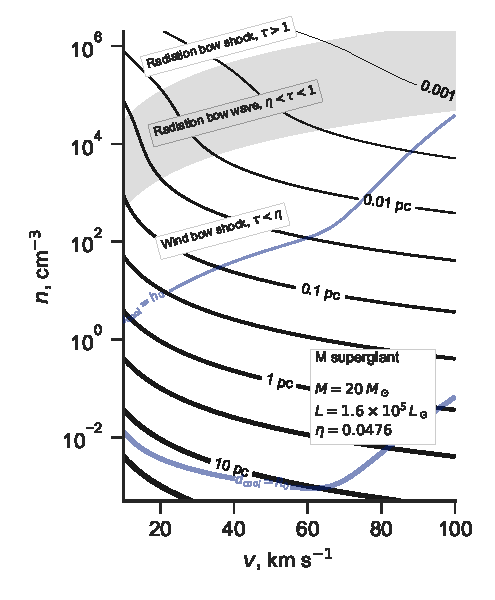
\includegraphics[width=\linewidth]{figs/zones-v-n-plane-RSG}
  \caption{As Fig.~\ref{fig:zones-v-n-plane}, but for a cool M-type
    supergiant instead of hot main sequence stars.  A smaller dust
    opacity is used, \(\kappa = \SI{60}{cm^2.g^{-1}}\), because of the
    reduced extinction efficiency at the optical/infrared wavelengths
    emitted by this star.}
  \label{fig:M-supergiant}
\end{figure}

It can be seen from Figure~\ref{fig:zones-v-n-plane} that the onset of
the radiation bow wave regime is very similar for the three
main-sequence stars, occurring at
\(n > \text{\numrange{20}{40}} \, v_{10}^2\).  An important
difference, however, is that for the \SI{40}{M_\odot} star, which has a
powerful wind, the radiation bow wave regime only occurs for a very
narrow range of densities, whereas for the \SI{10}{M_\odot} star, with a
much weaker wind, the regime is much broader, extending to
\(n < \num{e4} \, v_{10}^2\).  Another difference is the size scale of
the bows in this regime, which is
\(R_0 = \text{\SIrange{0.001}{0.003}{pc}}\) for the \SI{10}{M_\odot} star
if \(v_\infty = \SI{40}{km.s^{-1}}\), but \(R_0 \approx \SI{0.1}{pc}\) for the
\SI{40}{M_\odot} star, assuming the same inflow velocity.

Figure~\ref{fig:M-supergiant} shows results for a cool M-type
super-giant star with stellar parameters inspired by Betelgeuse
(\chemalpha~Orionis), as listed in Table~\ref{tab:stars}.  Unlike the
UV-dominated spectrum of the hot stars, this star emits predominantly
in the near-infrared, where the dust extinction efficiency is lower \citep{Weingartner:2001a},
so we adopt a lower opacity of \SI{60}{cm^2.g^{-1}}.  This has the
effect of shifting the radiation bow wave regime to higher densities:
\(n = \text{\numrange{1000}{30 000}}\, v_{10}^2\) in this case.


\subsection{Effects of stellar gravity}
\label{sec:effects-gravity}

In principle, gravitational attraction from the star, of mass \(M\),
will partially counteract the radiative acceleration.  This can be
accounted for by replacing \(L\) with an effective luminosity
\newcommand\Edd{\ensuremath{_{\text{E}}}}
\begin{equation}
  \label{eq:effective-luminosity}
  L_{\text{eff}} = L \bigl(1 - \Gamma\Edd^{\,-1}\bigr) \ ,
\end{equation}
in which \(\Gamma\Edd\) is the Eddington factor:
\begin{equation}
  \label{eq:eddington-factor}
  \Gamma\Edd = \frac{\kappa L}{4\pi c G M} = 458.5 \, \frac{\kappa_{600} L_4}{ M } \ ,
\end{equation}
where, in the last expression, \(M\) is measured in solar masses.  For
the stars in Table~\ref{tab:stars}, we find
\(\Gamma\Edd \approx \text{\numrange{30}{400}}\), so gravity can be safely
ignored.  When the optical depth of the bow is very large,
\(\tau > \ln\Gamma\Edd \sim 5\), gravity will exceed the radiation force in the
outer parts of the shell (see \citealt{Rodriguez-Ramirez:2016b}), but
it is generally too weak to affect the shell structure even in such a
case, see \S~\ref{sec:axial-structure-bow} below.


\section{Physical state of the bow shell}
\label{sec:phys-state-shock}

There are two shocked zones in the bow: an inner zone of shocked
stellar wind, and an outer zone of decelerated ambient stream. For OB
stars, dust grains are present only in the ambient stream, whereas for
cool stars they will also be present in the stellar wind.  In the
remainder of this paper, we will concentrate on the OB star case,
where it is the outer zone that is most important observationally.
Bows are typically detected via their infrared radiation (absorption
and re-emission by dust of stellar radiation), or by emission lines
such as the hydrogen H\(\alpha\) line.

% In the WBS and RBW case, this is also shocked

\subsection{Ionization state}
\label{sec:trapp-ioniz-front}

\begin{figure}
  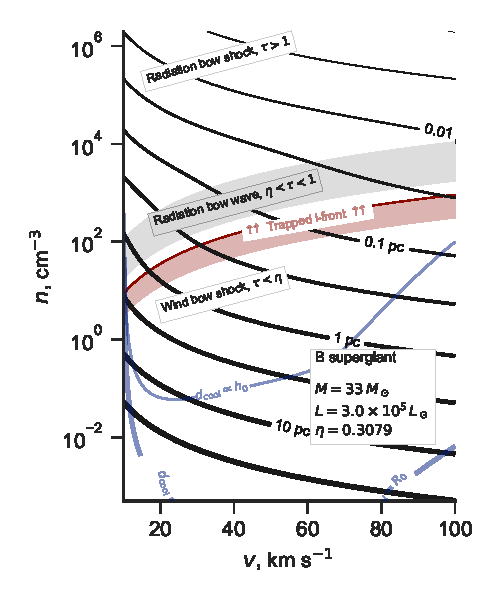
\includegraphics[width=\linewidth]{figs/zones-v-n-plane-BSG}
  \caption{As Fig.~\ref{fig:zones-v-n-plane}, but for an evolved
    B-type supergiant instead of main sequence stars.  This is similar
    to the early O MS star of Fig.~\ref{fig:zones-v-n-plane}\textit{c}
    in many respects, except for the trapping of the ionization front,
    which occurs for much lower outer stream densities.}
  \label{fig:B-supergiant}
\end{figure}

In this section we calculate whether the star is capable of
photoionizing the entire bow shock shell, or whether the ionization
front will be trapped within it.  Using the on-the-spot approximation
for the diffuse fields \citep{Osterbrock:2006a}, the number of
hydrogen recombinations per unit time per unit area in a fully ionized
shell of density \(n\shell\) and thickness \(h\shell\) is
\begin{equation}
  \label{eq:shell-recombination-rate}
  \mathcal{R} = \alphaB n\shell^2 h\shell \ ,
\end{equation}
where \(\alphaB = \num{2.6e-13}\, T_4^{-0.7}\, \si{cm^3.s^{-1}}\) is
the case~B recombination coefficient and \(T_4 = T/\SI{e4}{K}\).
The advective flux of hydrogen nuclei through the shock is
\begin{equation}
  \label{eq:shell-advective-flux}
  \mathcal{A} = n v_\infty \ ,
\end{equation}
and the flux of hydrogen-ionizing photons
(\(h \nu > \SI{13.6}{eV}\)) incident on the inner edge of the shell is
\begin{equation}
  \label{eq:shell-ionizing-flux}
  \mathcal{F} = \frac{S} {4 \pi R_0^2} \ , 
\end{equation}
where \(S\) is the ionizing photon luminosity of the star.  Any shell
with \(\mathcal{R} + \mathcal{A} > \mathcal{F}\) cannot be entirely
photoionized by the star, and so must have trapped the ionization
front.

The ratio of advective particle flux to ionizing flux is, from
equations~\eqref{eq:Rstar}, \eqref{eq:shell-advective-flux},
\eqref{eq:shell-ionizing-flux},
\begin{equation}
  \label{eq:advective-over-ionizing-flux}
  \frac{\mathcal{A}}{\mathcal{F}} = \num{5.86e-5} \frac{x^2 L_4}{v_{10} S_{49}} \ , 
\end{equation}
where
\begin{equation*}
  S_{49} = S / \bigl( \SI{e49}{s^{-1}} \bigr) \ .
\end{equation*}
Numerical values of \(S_{49}\) for our three example stars are given
in Table~\ref{tab:stars}, taken from Figure~4 of
\citet{Sternberg:2003a}.  Since \(\mathcal{A} \ll \mathcal{F}\) in
nearly all cases, for clarity of exposition we ignore \(\mathcal{A}\)
in the following discussion, although it is included in quantitative
calculations.  The column density of the shocked shell can be found,
for example, from equations~(10) and~(12) of \citet{Wilkin:1996a} in
the limit \(v_\infty/V \to 0\) (Wilkin's parameter \(\alpha\)) and
\(\theta \to 0\).  This yields
\begin{equation}
  \label{eq:shocked-shell-column}
  n\shell h\shell = \tfrac34 n R_0 \ .
\end{equation}
Assuming strong cooling behind the shock
(\S~\ref{sec:radi-cool-lengths}), the shell density is
\begin{equation}
  \label{eq:isothermal-shell-density}
  n\shell = \mathcal{M}_0^2 n \,
\end{equation}
where
\(\mathcal{M}_0 = v_\infty / \sound\) is the isothermal Mach number of the
external stream.\footnote{%
  \label{fn:temperature-dependence}
  The sound speed depends on the temperature and hydrogen and helium
  ionization fractions, \(y\) and \(y_{\text{He}}\) as
  \(\sound^2 = (1 + y + z_{\text{He}} y_{\text{He}}) (k T /
  \bar{m})\), where \(z_{\text{He}}\) is the helium nucleon abundance
  by number relative to hydrogen and
  \(k = \SI{1.3806503e-16}{erg.K^{-1}}\) is Boltzmann's constant.  We
  assume \(y = 1\), \(y_{\text{He}} = 0.5\), \(z_{\text{He}} = 0.09\),
  so that \(\sound = \num{11.4}\, T_4^{1/2}\, \si{km.s^{-1}}\). } %
Putting these together with equations~\eqref{eq:Rstar} and
~\eqref{eq:tau-star}, one finds that \(\mathcal{R} > \mathcal{F}\)
implies
\begin{equation}
  \label{eq:ifront-trap-x-cubed-taustar}
  x^3 \tau_* > \frac{4 S c \sound^2 \bar{m}^2 \kappa}{3 \alpha L} \ .
\end{equation}
From equation~\eqref{eq:rad-full-x}, it can be seen that \(x\) depends
on the external stream parameters, \(n\), \(v_\infty\) only via
\(\tau_*\), and so equation~\eqref{eq:ifront-trap-x-cubed-taustar} is a
condition for \(\tau_*\), which, by using
equation~\eqref{eq:taustar-typical}, becomes a condition on
\(n / v_{10}^2\).  In the radiation bow shock case,
\(x = (1 + \eta\wind)^{1/2}\), and the condition can be written:
\begin{equation}
  \label{eq:ifront-trap-density-RBS}
  \text{RBS:}\quad
  \frac{n}{v_{10}^2} > \num{2.65e8} \, \frac{S_{49}^2 T_4^{3.4}}{L_4^3 (1 + \eta\wind)^3} \ .
\end{equation}
In the radiation bow wave case, \(x = 2\tau_*\), and the condition can be
written:
\begin{equation}
  \label{eq:ifront-trap-taustar-RBW}
  \text{RBW:}\quad
  \frac{n}{v_{10}^2} > \num{5.36e4} \, \frac{S_{49}^{1/2} T_4^{0.85} }{\kappa_{600}^{3/2} L_4^{3/2}} \ . 
\end{equation}
In the wind bow shock case, the result is the same as
equation~\eqref{eq:ifront-trap-density-RBS}, but changing the factor
\((1 + \eta\wind)^3\) to \(\eta\wind^3\).  For the example hot stars in
Table~\ref{tab:stars}, and assuming \(\kappa_{600} = 1\),
\(T_4 = 0.8\), the resulting density threshold is
\(n > (\text{\numrange{1000}{5000}})\, v_{10}^2\), depending only
weakly on the stellar parameters, which is shown by the red lines in
Figure~\ref{fig:zones-v-n-plane}.  For the \SI{10}{M_\odot} star this is
in the radiation bow wave regime, whereas for the higher mass stars it
is in the radiation bow shock regime.  When the external stream is
denser than this, then the outer parts of the shocked shell may be
neutral instead of ionized, giving rise to a cometary compact \hii{}
region \citep{Mac-Low:1991a, Arthur:2006a}.  This is only necessarily
true, however, when the star is isolated.  If the star is in a cluster
environment, then the contribution of other nearby massive stars to
the ionizing radiation field must be considered.

Quite different results are obtained for a B-type supergiant star (see
Tab.~\ref{tab:stars} and Fig.~\ref{fig:B-supergiant}), which has a
similar bolometric luminosity and wind strength to the \SI{40}{M_\odot}
main-sequence star, but a hundred times lower ionizing luminosity.
This results in a far lower threshold for trapping the ionization
front of \(n > 40 v_{10}^2\).  The advective flux, \(\mathcal{A}\), is
relatively stronger for this star than for the main-sequence stars, but
even for \(v_{10} < 2\), where the effect is strongest, the change is
only of order the thickness of the dark red line in
Figure~\ref{fig:B-supergiant}.


In principle, when the ionization front trapping occurs in the bow
wave regime, then the curves for \(R_0\) will be modified in the
region above the red line because all of the ionizing radiation is
trapped in the shell due to gas opacity, which is not included in
equation~\eqref{eq:tau-thin}.  However, this only happens for our
\SI{10}{M_\odot} star, which has a relatively soft spectrum.
Table~\ref{tab:stars} gives the peak wavelength of the stellar
spectrum for this star as \(\lambda_{\text{eff}} = \SI{0.115}{\um}\), which
is significantly larger than the hydrogen ionization threshold at
\SI{0.0912}{\um}, meaning that only a small fraction of the total
stellar luminosity is in the EUV band and affected by the gas opacity.
The effect on \(R_0\) is therefore small.  For the higher mass stars,
\(\lambda_{\text{eff}} < \SI{0.0912}{\um}\), so the majority of the
luminosity is in the EUV band, but in these cases the ionization front
trapping occurs well inside the radiation bow shock zone, where the
dust optical depth is already sufficient to trap all of the radiative
momentum.

\subsection{Efficiency of radiative cooling}
\label{sec:radi-cool-lengths}
%
In this section, we calculate whether the radiative cooling is
sufficiently rapid behind the bow shock to allow the formation of a
thin, dense shell.  In general, cooling is least efficient at low
densities, so we will assume that the wind bow shock regime applies
unless otherwise specified. We label quantities just outside the shock
by the subscript ``0'', quantities just inside the shock (after
thermalization, but before any radiative cooling) by the subscript
``1'', and quantities after the gas has cooled back to the
photoionization equilibrium temperature by the subscript ``2''.
Assuming a ratio of specific heats, \(\gamma = 5/3\), the relation between
the pre-shock and immediate post-shock quantities
\citep{ZelDovich:1967} is
\begin{align}
  % \M_1 &= \left(\frac{\M_0^2 + 3} {5\M_0^2 - 1}\right)^{1/2} \\
  \label{eq:shock-n-jump}
  \frac{n_1}{n_0} &= \frac{4 \M_0^2} {\M_0^2 + 3} \\
  \label{eq:shock-T-jump}
  \frac{T_1}{T_0} &= \tfrac1{16} \bigl( 5\M_0^2 - 1 \bigr) \bigl( 1 + 3/\M_0^2 \bigr) \\
  \label{eq:shock-v-jump}
  \frac{v_1}{v_0} &= \left(\frac{n_1}{n_0}\right)^{-1} \ ,
\end{align}
where \(\M_0 = v_0 / \sound\).  The cooling length of the post-shock
gas can be written as
\newcommand\cool{\ensuremath{_{\text{cool}}}}
\begin{equation}
  \label{eq:dcool}
  d\cool = \frac{3 P_1 v_1} { 2 \bigl(  \mathcal{L}_1 - \mathcal{G}_1 \bigr) }\ ,  
\end{equation}
where \(P_1\) is the thermal pressure and \(\mathcal{L}_1\),
\(\mathcal{G}_1\) are the volumetric radiative cooling and heating
rates.  For fully photoionized gas, we have
\(P_1 \approx 2 n_1 k T_1\), \(\mathcal{L}_1 = n_1^2 \Lambda(T_1)\), and
\(\mathcal{G}_1 = n_1^2 \Gamma(T_1)\), where \(\Lambda(T)\) is the cooling
coefficient, which is dominated by metal emission lines that are
excited by electron collisions, and \(\Gamma(T)\) is the heating
coefficient, which is dominated by hydrogen photo-electrons
\citep{Osterbrock:2006a}. The cooling coefficient has a maximum around
\SI{e5}{K}, and for typical ISM abundances can be approximated as
follows:
\begin{align}
  \label{eq:cooling-coefficient}
  \Lambda_{\text{warm}} &= \num{3.3e-24} \, T_4^{2.3} \, \si{erg.cm^{3}.s^{-1}}\\
  \Lambda_{\text{hot}} &= \num{e-20} \, T_4^{-1}\, \si{erg.cm^{3}.s^{-1}} \\
  \Lambda &= \left( \Lambda_{\text{warm}}^{-k} +  \Lambda_{\text{hot}}^{-k} \right)^{-1/k}
      \quad \text{with} \quad k = 3 \ ,
\end{align}
which is valid in the range \(0.7 < T_4 < 1000\).  We approximate the heating coefficient as
\begin{equation}
  \label{eq:heating-coefficient}
  \Gamma = \num{1.77e-24} \, T_4^{-1/2} \, \si{erg.cm^{3}.s^{-1}} \ ,
\end{equation}
where the coefficient is chosen so as to give \(\Gamma = \Lambda\) at
an equilibrium temperature of \(T_4 = 0.8\).

In Figure~\ref{fig:zones-v-n-plane} we show curves calculated from
equations~\eqref{eq:shock-n-jump} to~\eqref{eq:heating-coefficient},
corresponding to \(d\cool = R_0\) (thick blue line) and
\(d\cool = h_0\) (thin blue line), where \(h_0\) is the shell
thickness in the limit of instantaneous cooling.  In this context,
\(n_0 = n\) and \(n_2 = n\shell\), so that \(h_0\) follows from
equations~\eqref{eq:shocked-shell-column}
and~\eqref{eq:isothermal-shell-density} as
\begin{equation}
  \label{eq:strong-cooling-h0}
  h_0 = \tfrac34 \M_0^{-2} R_0 \ .
\end{equation}
The bends in the curves at \(v \approx \SI{50}{km.s^{-1}}\) are due to the
maximum in the cooling coefficient \(\Lambda(T)\) around
\(\SI{e5}{K}\).  For bows with outer stream densities above the thin
blue line, radiative cooling is so efficient that the bow shock can be
considered isothermal, and so the shell is dense and thin (at least,
in the apex region).  It can be seen that the ionization front
trapping always occurs at densities larger than this, which justifies
the use of equation~\eqref{eq:isothermal-shell-density} in the
previous section.  For bows with outer stream densities below the
thick blue line, cooling is unimportant and the bow shock can be
considered non-radiative.  In this case the shell is thicker than in
the radiative case,
\(h\shell/R_0 \approx \text{\numrange{0.2}{0.3}}\).  This value can be found
from equation~\eqref{eq:shocked-shell-column} by substituting
\(n = n_0\) and \(n\shell \approx 1.1 n_1\), then using
equation~\eqref{eq:shock-n-jump}. The factor \num{1.1} comes from
consideration of the slight increase in density between the shock and
the contact/tangential discontinuity.  For bows with outer stream
densities between the two blue lines, cooling does occur, albeit
inefficiently, so that the shell thickness \(h\shell\) is set by
\(d\cool\) rather than \(h_0\).

\subsection{Axial structure of bow shells}
\label{sec:axial-structure-bow}

\begin{figure}
  \centering
  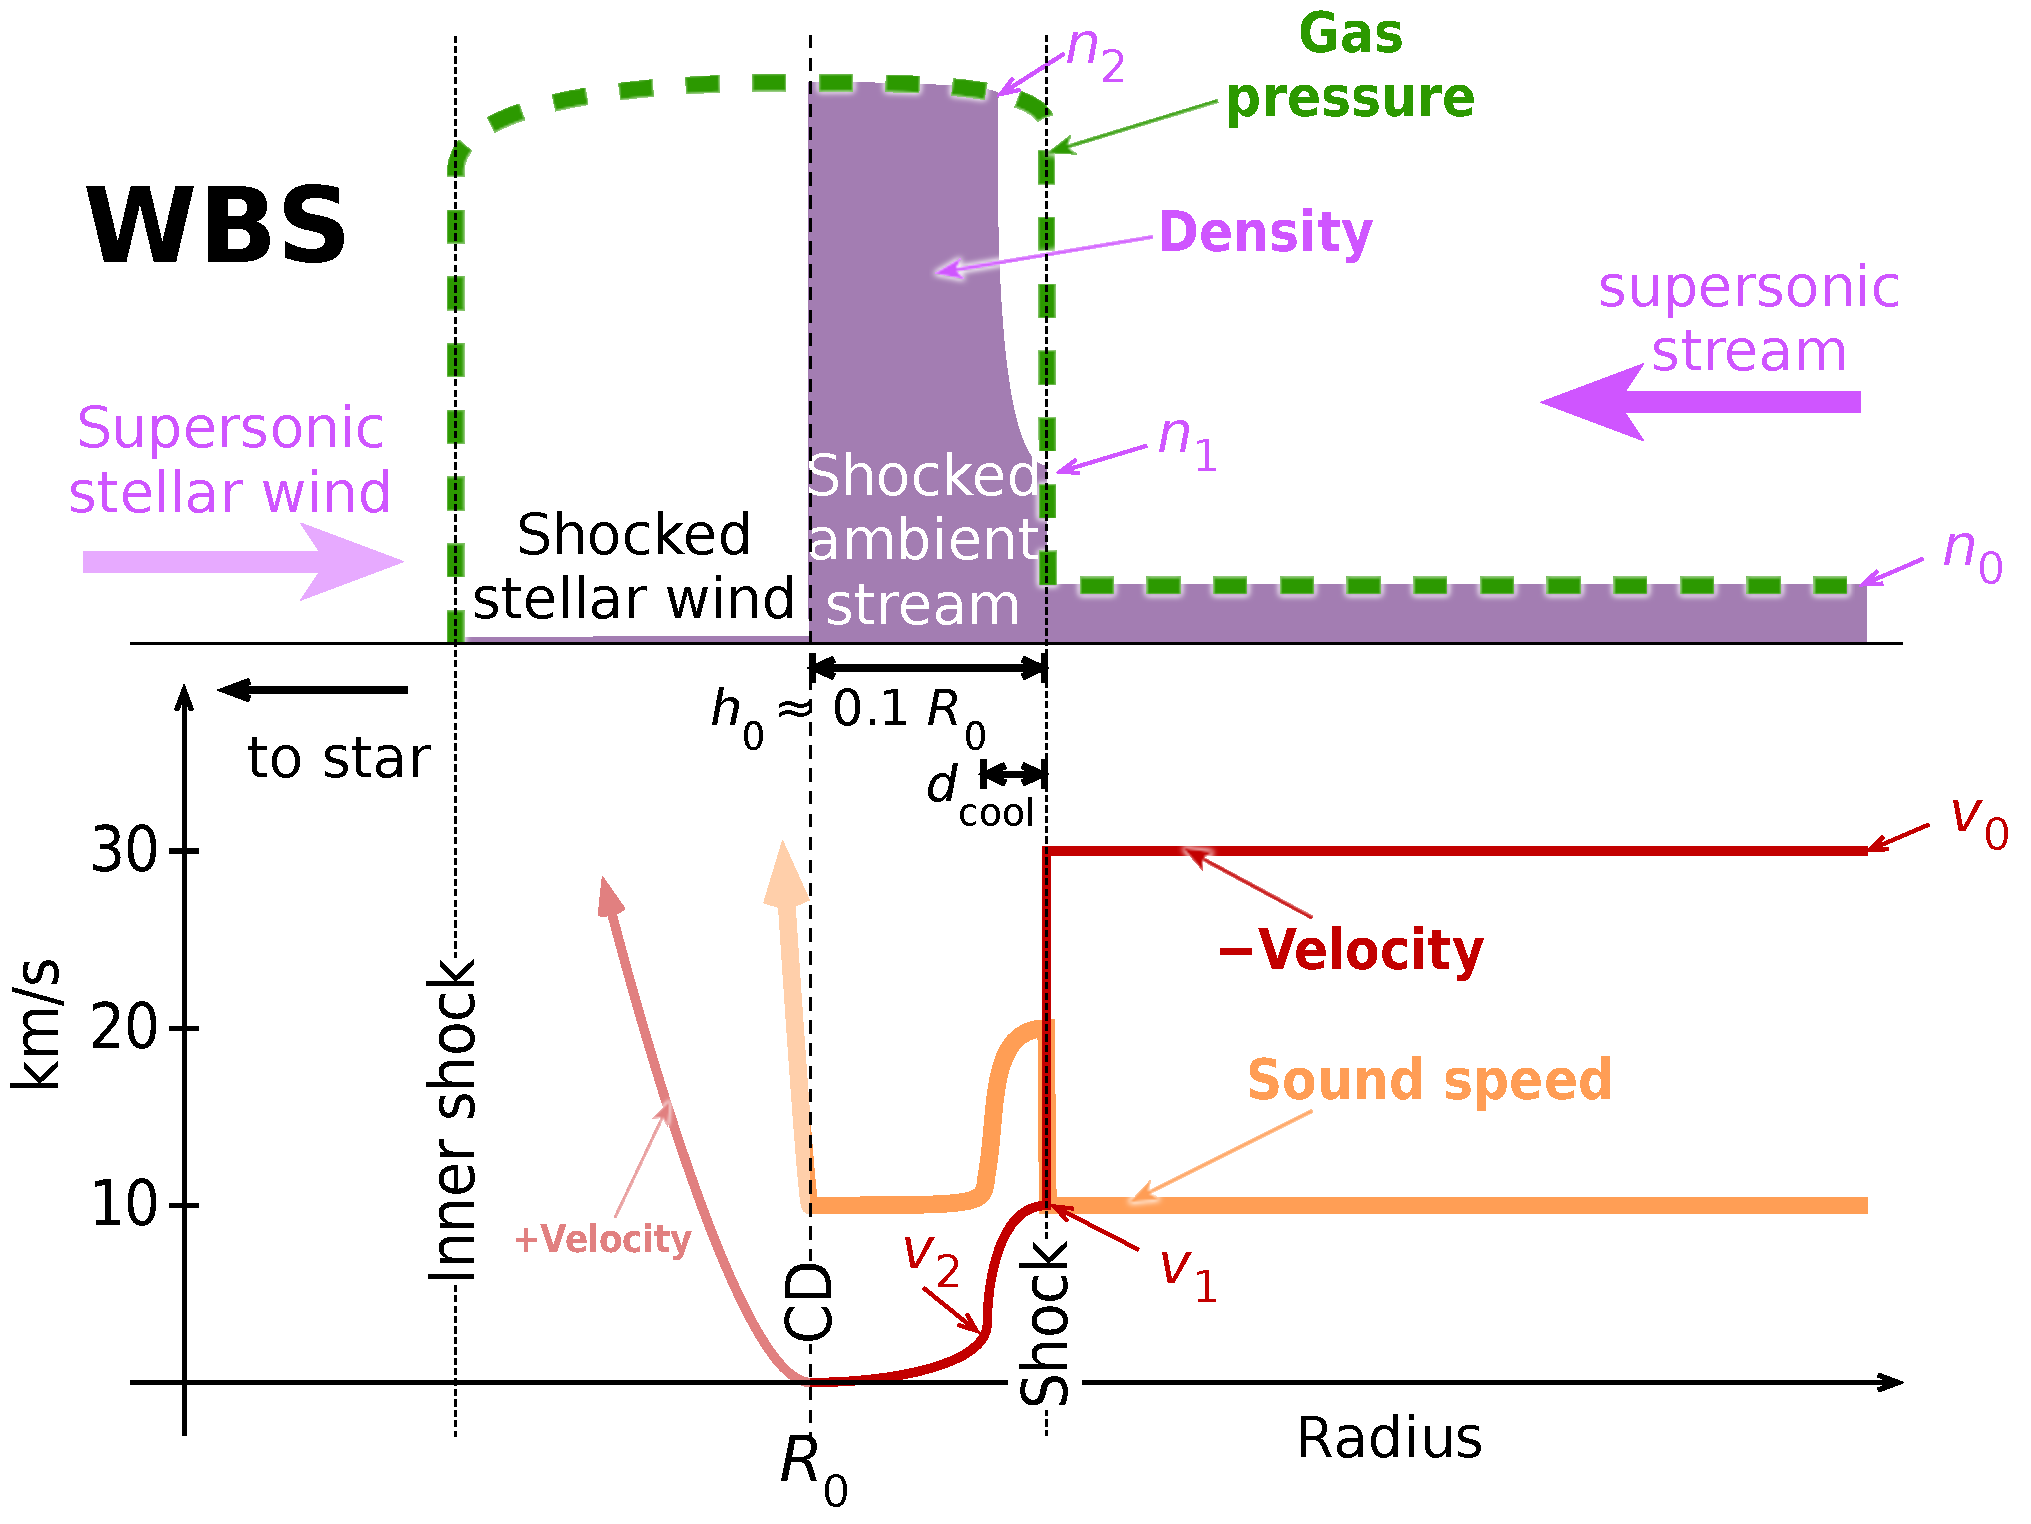
\includegraphics[width=\linewidth]{figs/shell-profile-wbs}
  \caption{Profiles of physical variables along the axis of the bow
    shell for a wind-supported bow shock.  The case is shown of a
    stream velocity of \SI{30}{km.s^{-1}} and an equilibrium ionized
    sound speed of \SI{10}{km.s^{-1}}.}
  \label{fig:axial-structure-wbs}
\end{figure}
\begin{figure}
  \centering
  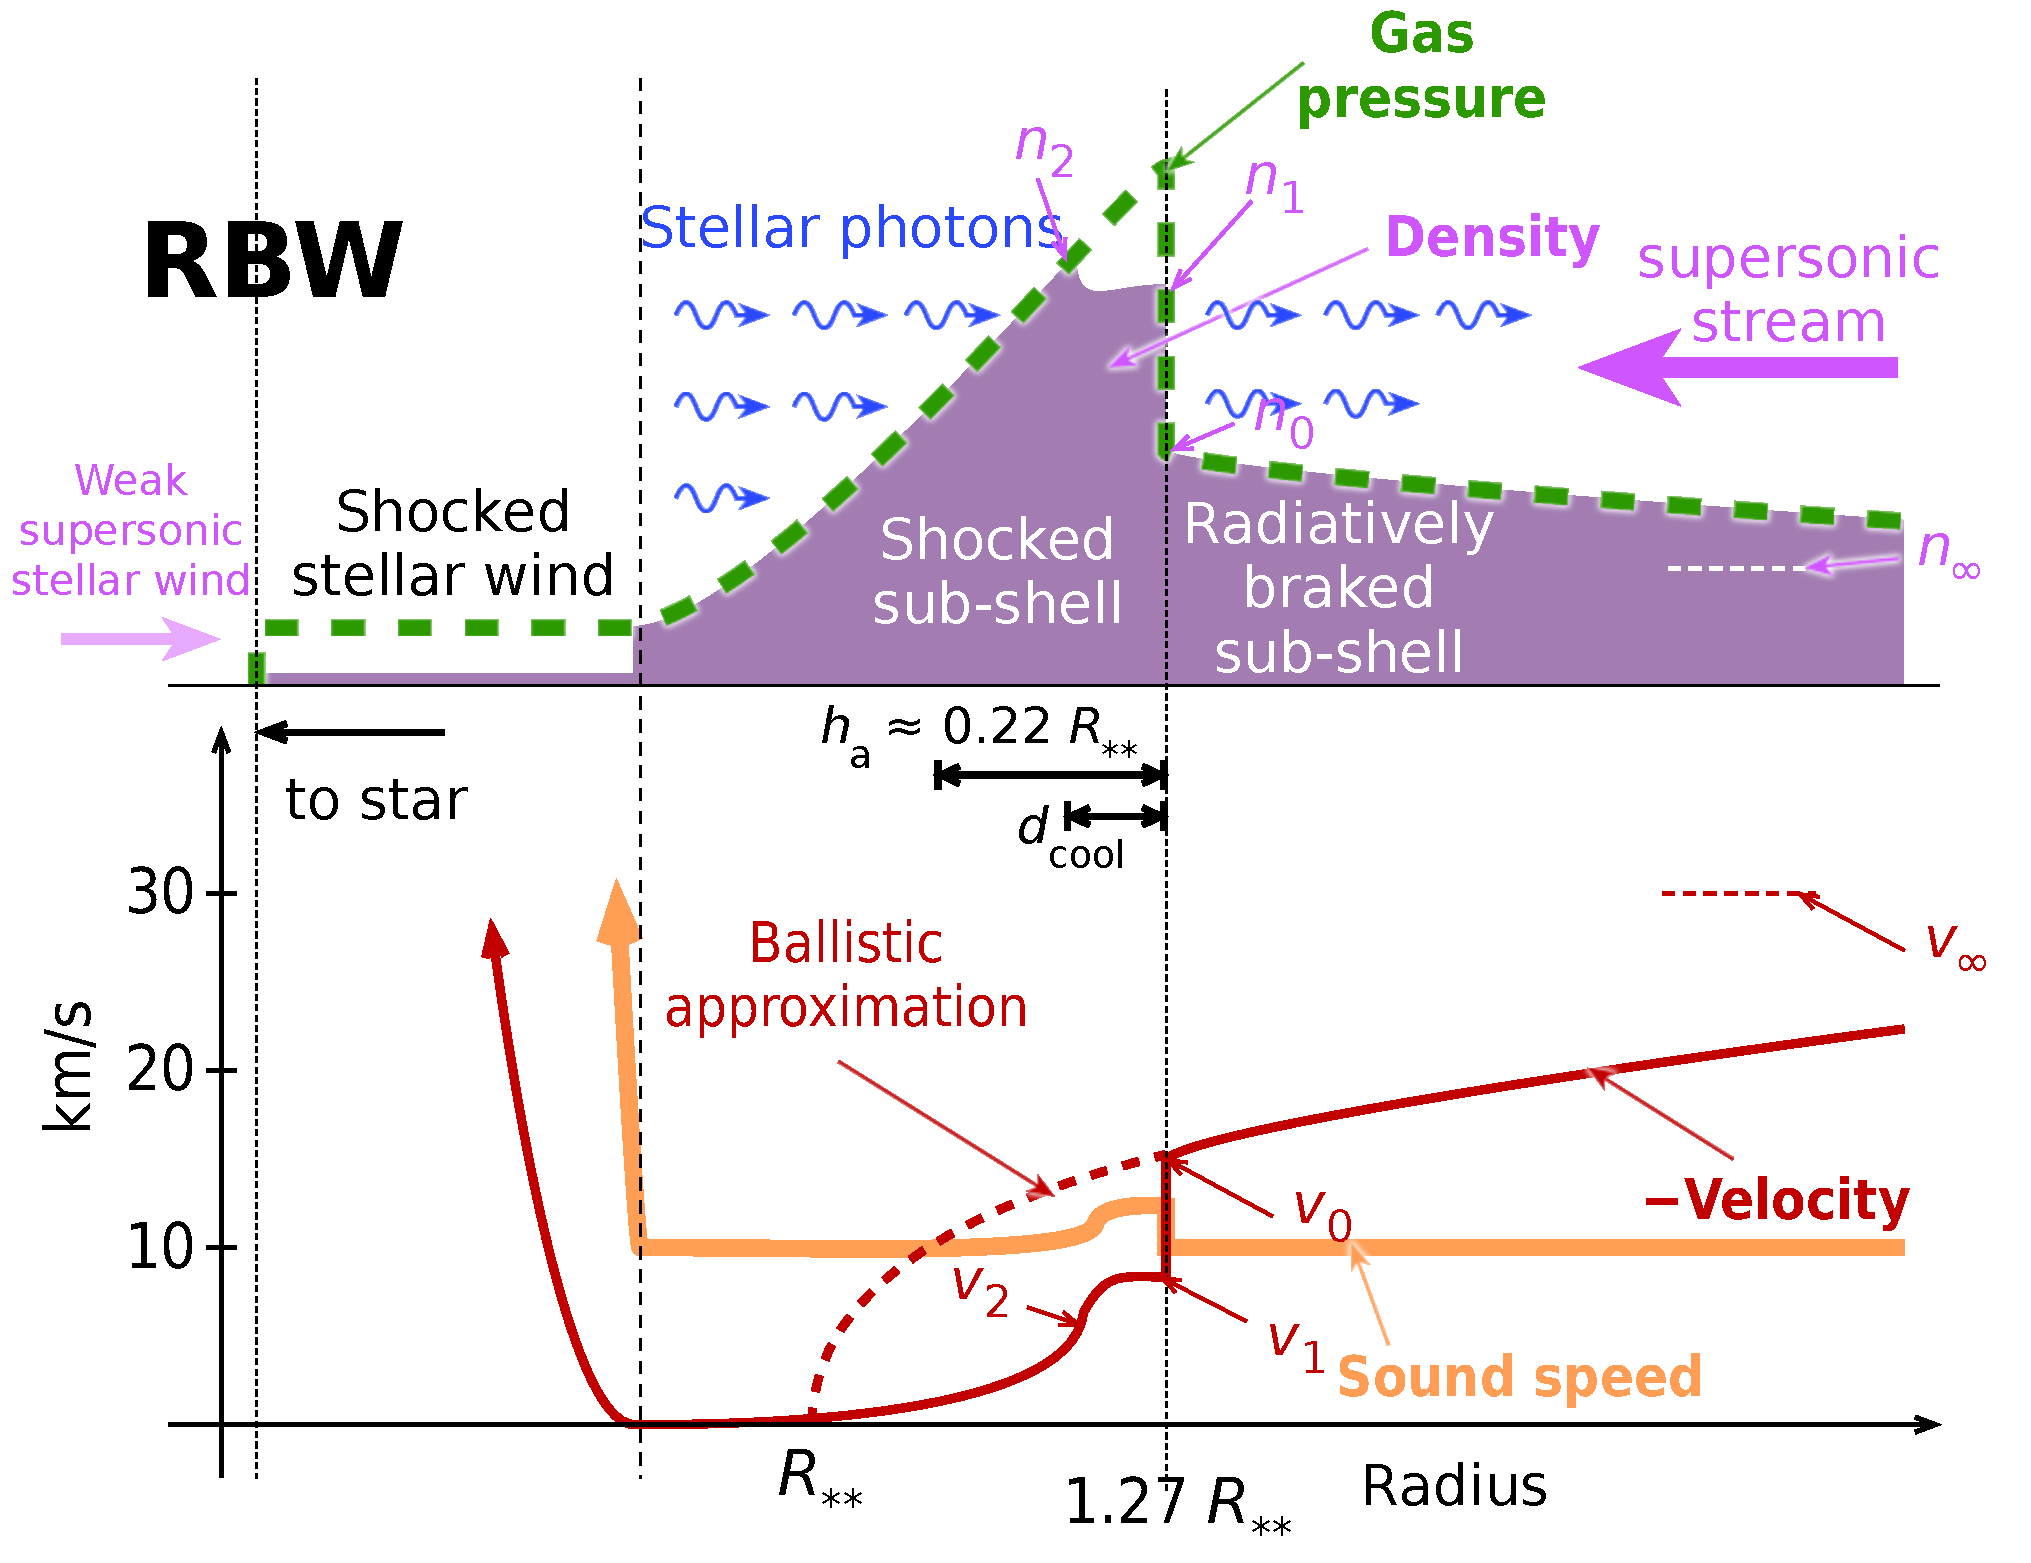
\includegraphics[width=\linewidth]{figs/shell-profile-rbw}
  \caption{As Fig.~\ref{fig:axial-structure-wbs} but for a
    radiation-supported bow wave.}
  \label{fig:axial-structure-rbw}
\end{figure}
\begin{figure}
  \centering
  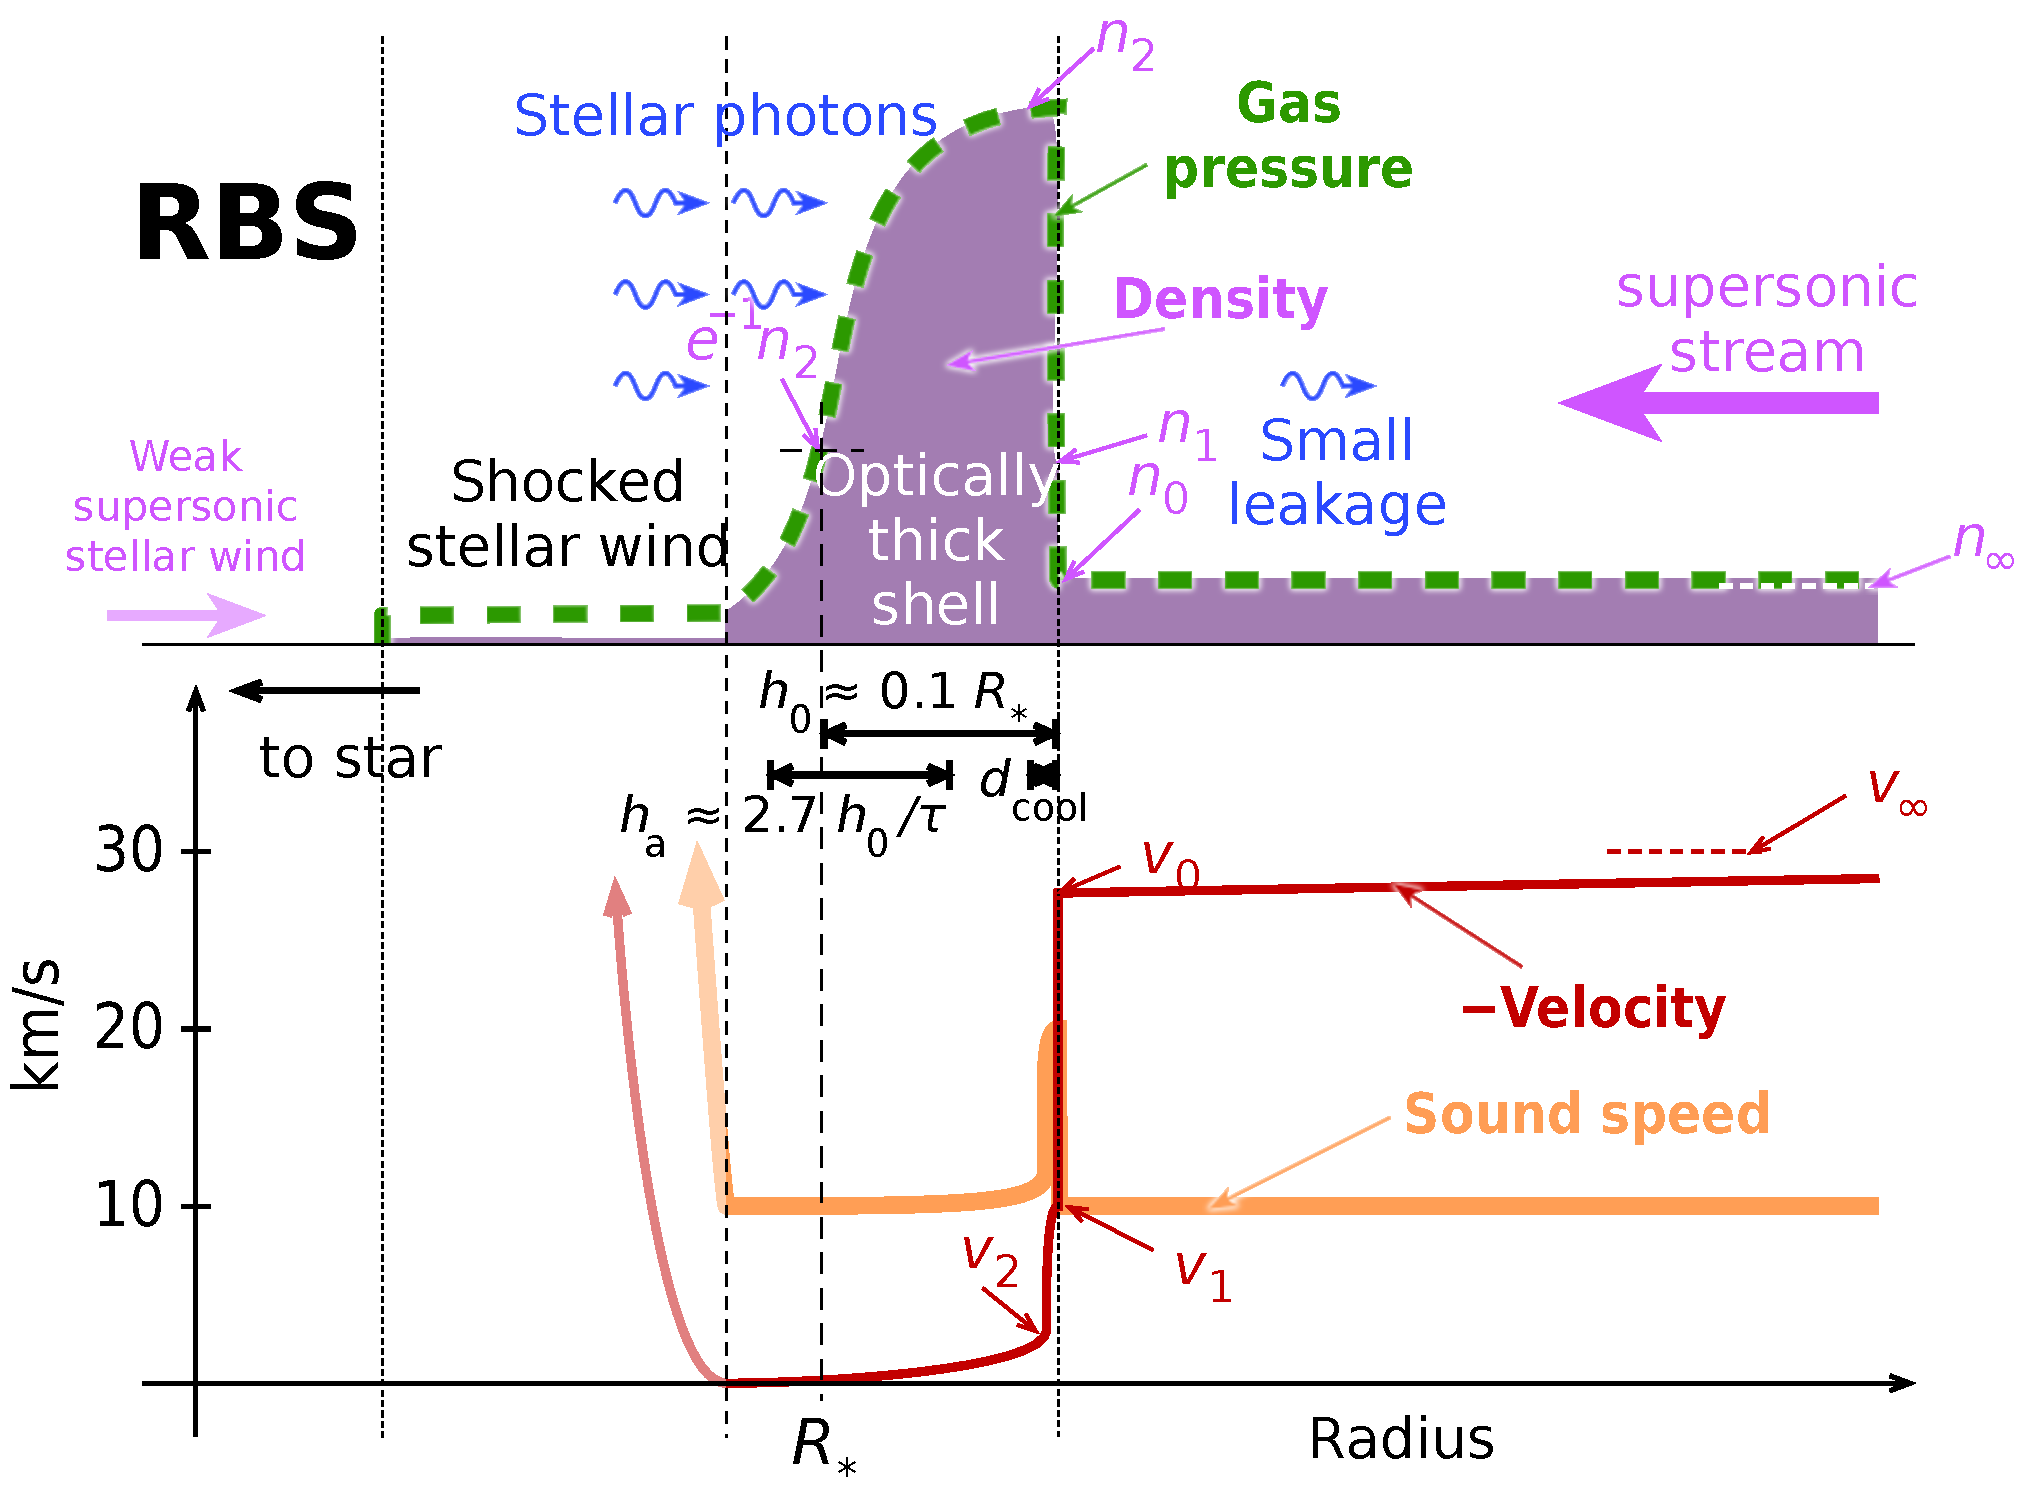
\includegraphics[width=\linewidth]{figs/shell-profile-rbs}
  \caption{As Fig.~\ref{fig:axial-structure-wbs} but for a
    radiation-supported bow shock.}
  \label{fig:axial-structure-rbs}
\end{figure}

In the shell of a wind-supported bow shock, the gas density is highest
at the contact discontinuity, but this is no longer true for
radiation-supported bows, as illustrated in
Figures~\ref{fig:axial-structure-wbs} to
\ref{fig:axial-structure-rbs}, where we schematically show the shell
structure for the three cases: WBS, RBW, and RBS.  In all cases, we
assume a far-field mach number of \(\M_\infty = 3\) for the incident stream
of density \(n_\infty\).  For the WBS case
(Fig.~\ref{fig:axial-structure-wbs}), the stream is unchanged until it
reaches the shock, so \(\M_0 = \M_\infty\) and \(n_0 = n_\infty\).  The density
increases to \(n_1 = 3 n_0\) in the shock
(eq.~[\ref{eq:shock-n-jump}]), and then to \(n_2 = 9 n_0\)
(eq.~[\ref{eq:isothermal-shell-density}]) after it has cooled back
down to the equilibrium photoionized temperature.  In the figure, we
show the case where \(d\cool < h_0\), so that most of the shell is at
roughly constant density.  Note that although the mass flux along the
axis, \(n v\), is approximately conserved in most of the flow, this is
no longer true close to the contact discontinuity, since the
streamlines bend away from the axis due to lateral pressure gradients.
This is what allows \(v\) to tend to zero, while \(n\) remains
constant.  The thermal pressure in the shocked stellar wind is equal
to the shell pressure, but its density is much smaller due to a
temperature that is higher by a factor of \(\approx 3100 V_3^2\),
(eq.~[\ref{eq:shock-T-jump}], assuming inefficient cooling).

For the optically thin RBW case (Fig.~\ref{fig:axial-structure-rbw}),
equations~\eqref{eq:rad-accel} to~\eqref{eq:rad:R0} can be combined to
give the radial dependence of the stream velocity as it approaches the
star:
\begin{equation}
  \label{eq:v-RBW-ballistic}
  v(R) = \left( 1 - \frac{R_{**}}{R} \right)^{1/2} v_\infty \ .
\end{equation}
This ballistic approximation (shown by the dashed red line in
Fig.~\ref{fig:axial-structure-rbw}) predicts that the velocity smoothly
decreases to zero at \(R = R_{**}\).  However, although this is valid
in the limit of high Mach number, it ignores the effects of gas
pressure and so becomes invalid once the stream velocity falls close
to the sound speed.  The situation bears similarities to the flow in a
supersonic diffuser, such as the inlet of a ramjet or other supersonic
aircraft engine \citep{Seddon:1999a}, which slows supersonic airflow
down to subsonic speeds before combustion.  Exactly the opposite flow
configuration is present in a rocket nozzle \citep{Courant:1948a},
where the flow can smoothly pass from subsonic to supersonic
velocities at the throat of the nozzle.  An analogy between an
isothermal stellar wind and a rocket nozzle is developed in detail in
\S~3.5 of \citet{Lamers:1999b}.  However, in the reverse case of a
supersonic diffuser, a smooth transition from supersonic to subsonic
flow is not possible \citep{Morawetz:1956a}.  Instead, a normal shock
wave develops, which decelerates the supersonically entering flow,
allowing it to exit subsonically \citep{Embid:1984a, Hafez:1999a}.
The supersonic inlet/bow wave analogy is not so exact as the rocket
nozzle/stellar wind analogy due to the multi-dimensional nature of the
bow shell, which means that lateral flows of gas away from the apex
become important when the velocity is subsonic.\footnote{%
  In the aeronautical case, the inlet is usually designed so that
  multiple oblique shocks partially decelerate the flow before it
  passes through the normal shock.  This is the analogy of the initial
  gradual radiative deceleration in the bow wave.  } %
Nonetheless, we expect that a normal shock must be present in the
flow, although there does not seem to be any simple argument for
predicting the exact Mach number where it will occur.  In
Figure.~\ref{fig:axial-structure-rbw} we assume that the shock occurs at
a Mach number \(\M_0 = 1.5\), but multidimensional numerical
simulations are necessary to test this supposition.

The shell in the RBW case therefore consists of two parts: an outer
radiatively braked sub-shell, and an inner shocked sub-shell.  In the
outer sub-shell, the density gradually increases inwards as the stream
is decelerated by the absorbed photons, reaching
\begin{equation}
  \label{eq:outer-shell-density}
  n_0 = \frac{\M_\infty}{\M_0} n_\infty
\end{equation}
just outside the shock (\(n_0 = 2 n_\infty\) for the case illustrated).  In
the inner sub-shell, on the other hand, the pressure must increase
outwards, since it is subsonic and therefore in approximate
hydrostatic equilibrium with an outward-pointing effective gravity
from the radiation force.  The shell thickness will be set by the
hydrostatic scale height, \(h_a = \sound^2 / a\rad\), which by
eqs.~(\ref{eq:rad-accel}, \ref{eq:rad:R0}) is given by
\begin{equation}
  \label{eq:scale-height}
  h_a = \frac{2 R_{**}}{\M_\infty^2} \ .
\end{equation}
If the cooling is efficient (\(d\cool < h_a\)), then most of the
sub-shell is isothermal and the density will fall off exponentially
towards the star.  The contact discontinuity with the stellar wind
will form at the point where the shell pressure has fallen by a factor
of order \(\tau / \eta\wind\), but this has no influence on the bulk of the
shell, which is pressurized by radiation, not wind.  If, as we
suspect, \(\M_0\) depends only weakly, if at all, on \(\M_\infty\), then
eqs.~(\ref{eq:outer-shell-density}, \ref{eq:scale-height}) imply that
the inner shocked sub-shell represents a fraction
\(\approx \M_\infty^{-1}\) of the total shell optical depth, which means that the
outer supersonic sub-shell dominates for highly supersonic stream
velocities.

For the optically thick RBS case (Fig.~\ref{fig:axial-structure-rbs}),
the shell density profile is no longer simply exponential since the
pressure scale height now increases as one moves away from the star,
due to the extinction-induced decline in radiation flux. Assuming
single scattering and plane geometry, the resultant hydrostatic
density profile is doubly exponential:
\begin{equation}
  \label{eq:rbs-density-profile}
  n(R) = n_2 e^{-e^{-x}} \text{\quad where\quad } x = n_2 \bar{m} \kappa (R - R_*) \ . 
\end{equation}
The shell density increases from \(e^{-1} n_2\) at \(R_*\) to saturate
at \(n_2\) for \(R > R_* + h_a\), where \(h_a\) is now the pressure
scale height at the inner edge of the shell.  From
equations~(\ref{eq:Rstar}, \ref{eq:rad:R0}, \ref{eq:tau-thin},
\ref{eq:strong-cooling-h0}, \ref{eq:scale-height}), and taking \(R_0 \approx R_*\), we find
\begin{equation}
  \label{eq:ha-versus-h0}
  h_a \approx \frac{4 h_0}{3 \tau} \ .
\end{equation}
We show results for a total shell optical depth \(\tau = 3\), for which
\(h_a\) is a significant fraction of \(h_0\).  For much larger optical
depths, \(h_0 \gg h_a\) so that the constant density portion of the
shell will dominate the total column.  A small fraction \(e^{-\tau}\) of
the photons will penetrate the shell and be available to decelerate
the supersonic stream, as in the RBW case, yielding
\(v_0 = (1 - \tau e^{-\tau})\, v_\infty\).  In the illustrated case of
\(\tau = 3\), the resultant speed reduction before the shock is only 8\%.
As mentioned in \S~\ref{sec:effects-gravity}, radiative acceleration
becomes less important than gravity in the outer regions of an opaque
shell.  However, in order for this to have a significant effect on the
shell, the gravitational scale height would have to be be less than
the shell thickness: \(\Gamma\Edd h_a < h_0\).  From
equation~\eqref{eq:ha-versus-h0} this translates to
\(\tau > \frac43 \Gamma\Edd\), where dust-opacity Eddington factors are
\(\Gamma\Edd \sim 100\) for OB stars.  Such large optical depths would
require extremely high ambient densities of
\(n > \num{2e7} L_4 \,v_{10}^2 \left( \SI{10}{M_\odot}/M \right)^2 \,
\si{cm^{-3}} \), where we have used equations~(\ref{eq:tau-star},
\ref{eq:eddington-factor}) and that \(\tau \approx 2\tau_*\) in the RBS limit.

\section{Discussion}
\label{sec:discussion}

The stellar bows modeled in this paper can be seen as either due to
the motion of a star through the interstellar medium, or due to the
motion of the interstellar medium that flows past the star.  The
first case corresponds to runaway stars \citep{Blaauw:1961a}, which
have been ejected from a binary system or stellar cluster
\citep{Hoogerwerf:2001a}, while the second case can be due to
photoevaporation and champagne flows in \hii{} regions
\citep{Tenorio-Tagle:1979a, Shu:2002a, Henney:2005a}, or to general
turbulent flows in the Galaxy
\citep[e.g.,][]{Ballesteros-Paredes:1999a}.  In this section, we
consider the stream densities and velocities expected in each of these
scenarios, and compare them with our predictions for the type of bows
that should result.

Although some runaway stars have velocities exceeding
\SI{100}{km.s^{-1}}, most are moving considerably slower, with a
median peculiar velocity of about \SI{30}{km.s^{-1}}
\citep{Tetzlaff:2011a}.  The higher velocity runaways are likely
produced by dynamical interactions in the center of young clusters
\citep{Gualandris:2004a}, whereas the supernova-induced dissolution of
binary systems is predicted to primarily produce ``walkaways'' with
even slower velocities of order \SI{10}{km.s^{-1}}
\citep{Renzo:2018a}.  Environmental flows are also expected to be of
order \SI{10}{km.s^{-1}}, which is a characteristic velocity
dispersion for warm neutral gas in the inner Galaxy
\citep{Marasco:2017a} and also a typical expansion velocity for
\ion{H}{i} shells \citep{Ehlerova:2005a}.  Internal velocity
dispersions within \hii{} regions are subsonic
(\SIrange{5}{10}{km.s^{-1}}) for small regions, such as the Orion
Nebula, containing one or a few ionizing stars
\citep{Arthur:2016a}. This increases slowly for more luminous regions
as \(\sigma \propto L^{1/4}\) \citep{Bordalo:2011a}, so giant star forming
complexes such as Carina (100 times more luminous than Orion) show
velocity dispersions of order \SI{20}{km.s^{-1}}
\citep{Damiani:2016a}.  Higher velocities of
\SIrange{30}{40}{km.s^{-1}} are reached in divergent photoevaporation
flows \citep{Dyson:1968a}, but this is achieved at expense of a lower
density.  Given all the above, we expect there to be many more bows
with relative stream velocity \(v_\infty \sim \SI{20}{km.s^{-1}}\) than bows
with \(v_\infty \sim \SI{100}{km.s^{-1}}\).

Turning now to the ambient density, if bow shock stars were randomly
sampling the volume of the Galactic disk, then we would expect the
average density to be \(< \SI{1}{cm^{-3}}\).  The dominant gas phase
\citep{Ferriere:2001a} near the Galactic mid-plane is the Warm Neutral
Medium with a volume filling fraction of 45\% \citep[Fig.~11
of][]{Kalberla:2009a} and an average density of \SI{0.9}{cm^{-3}} at
the Solar circle \citep[\S~4 of][]{Kalberla:2008a}.  Significant
fractions of the volume (\(\approx 20\%\) each) are also occupied by the
Warm Ionized Medium and Hot Ionized Medium, which have even lower
densities (\(\approx \SI{0.3}{cm^{-3}}\) and \SI{e-3}{cm^{-3}},
respectively) and which increasingly dominate the volume for heights
\(z > \SI{500}{pc}\) above the plane.  The denser Cold Neutral Medium
(\(n \approx \text{\SIrange{10}{100}{cm^{-3}}}\)) and Molecular Clouds
(\(n > \SI{1000}{cm^{-3}}\)) occupy much smaller volumes
(\(\approx 10\%\) and \(< 1\%\), respectively).  However, observations of
stellar bows are clearly biased towards these higher densities.

In part, this bias is due to bows being easier to detect in denser
environments.  Depending on the emission mechanism, the shell
luminosity will be proportional to the column density
(\(\propto n R_0\)) or volume emission measure
(\(\propto n^2 R_0^3\)), which are both increasing functions of \(n\) since,
from \S~\ref{sec:three-bow-regimes}, the bow size falls relatively
slowly as \(R_0 \propto n^{-1/2}\) in the WBS and RBS cases, and is
independent of \(n\) in the RBW case.  Another contribution to the
high-density bias is simply that none but the highest velocity
high-mass stars can move far during their lifetime from the molecular
clouds where they were born.  Even a runaway star with
\(v = \SI{30}{km.s^{-1}}\), will travel \(< \SI{120}{pc}\) during an
O-star lifetime of \(< \SI{4}{Myr}\), which is of the same order as
the sizes of Giant Molecular Clouds.  Many observed stellar bows are
found in high mass star clusters associated with large \hii{} regions
\citep{Povich:2008a, Sexton:2015b}.  The ionized gas density in
Carina, for example, has an average value of
\(\approx \SI{100}{cm^{-3}}\) \citep{Oberst:2011a, Damiani:2016a}, although
with peaks \(> \SI{3000}{cm^{-3}}\) in photoevaporation flows from
embedded molecular globules \citep{Smith:2004a}.  In more compact
\hii{} regions, such as the Orion Nebula, ionized densities up to
\SI{e4}{cm^{-3}} are found on scales of about \(\SI{0.1}{pc}\)
\citep{Weilbacher:2015a, ODell:2017b}.

In \S~\ref{sec:depend-stell-type} we found that the bow is
wind-supported when \(\tau_*^2 < \eta\wind\), where \(\tau_*\) is a fiducial
optical depth (eq.~[\ref{eq:taustar-typical}]) and \(\eta\wind\) is the
radiative momentum efficiency of the stellar wind
(eq.~[\ref{eq:wind-eta-typical}]).  This translates into a maximum
stream density for wind-supported bows of
\newcommand\crit{\ensuremath{_{\text{max}}}}
\newcommand\vink{\ensuremath{_{\text{\tiny Vink}}}}
\begin{equation}
  \label{eq:ncrit}
  n\crit \approx \left(\SI{30}{cm^{-3}}\right)
  \left(  \frac{v} {\SI{10}{km.s^{-1}}}\right)^2
  \left( \frac{\eta\wind}{\eta\vink} \right)
  \left( \frac{\SI{600}{cm^2.g^{-1}}}{\kappa} \right)
  \ ,
\end{equation}
which is largely insensitive to spectral type between early-B and
early-O stars.  In this equation, we have expressed the wind
efficiency in terms of the Table~\ref{tab:stars} values,
\(\eta\vink\), which are calculated from the \citet{Vink:2000a} recipe,
and the UV dust opacity in terms of the standard ISM value adopted in
\S~\ref{sec:depend-stell-type}.

Therefore, runaway stars moving through the diffuse ISM with
\(n \sim \SI{1}{cm^{-3}}\) and \(v \sim \SI{30}{km.s^{-1}}\) are safely in
the WBS regime, having \(n \approx \num{0.004}\, n\crit\) for the default
wind and dust parameters.  On the other hand, slow-moving stars in
\hii{} regions of moderate density (\(n \sim \SI{100}{cm^{-3}}\)) can
easily have \(n > n\crit\), meaning that their bows will be radiation
supported.

\begin{figure}
  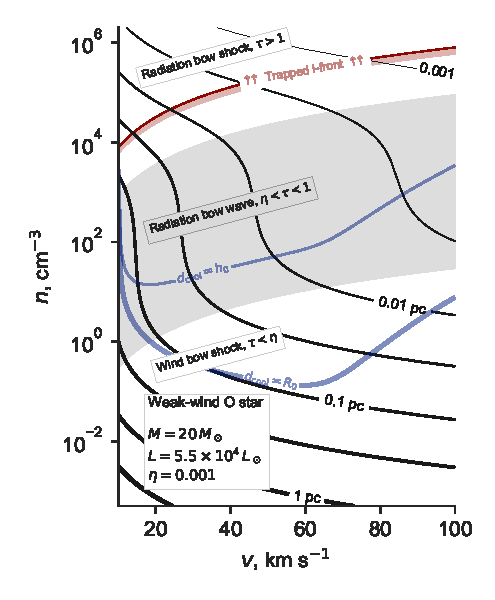
\includegraphics[width=\linewidth]{figs/zones-v-n-plane-Weak}
  \caption{As Fig.~\ref{fig:zones-v-n-plane}, but for a weak-wind
    O~star, similar to the sample observed by \citet{Martins:2005b}.
    For this star, radiation-supported bow waves (gray shading) occur
    over a much larger region of parameter space than for a
    normal-wind star of the same spectral type
    (see Fig.~\ref{fig:zones-v-n-plane}b).}
  \label{fig:O-weak-wind}
\end{figure}


For cases where the stellar wind or dust properties differ from our
assumed values, then these conclusions may change.  For instance,
there are a growing number of stars for which very low mass-loss rates
have been diagnosed from UV, optical or infrared line profiles
\citep{Martins:2005b, Marcolino:2009a, Najarro:2011a, Martins:2012a,
  Shenar:2017a, Smith:2017b}.  Most of these stars are late-type
O~dwarfs, for which the \citet{Vink:2000a} prescription predicts a
mass-loss rate of \num{3e-8} to \SI{e-7}{M_\odot.yr^{-1}}, whereas the
observationally derived values are in the range \num{e-10} to
\SI{3e-9}{M_\odot.yr^{-1}} -- a shortfall of 10 to 1000!  This ``weak wind
problem'' is a far larger discrepancy than can be explained by
clumping effects.  A potential (partial) resolution is to suppose that
internal shocks near the base of the wind, together with thermal
conduction, heat a large fraction of the gas to coronal temperatures,
where it is no longer detectable by means of standard wind diagnostic
lines \citep{Lucy:2012a}.  However, in cases where x-ray diagnostics
have been used to trace the mass loss of this hot component
(\(\mu\)~Col, \citealp{Huenemoerder:2012a}; \(\zeta\)~Oph,
\citealp{Cohen:2014a}), rates that are still an order of magnitude
below the Vink values are found (see also \citealp{Shenar:2017a}).  In
Figure~\ref{fig:O-weak-wind}, we show results for a weak-wind O9
dwarf, which is identical to the \SI{20}{M_\odot} star from
Table~\ref{tab:stars}, except with \(\eta\wind = 0.01 \eta\vink\)
(approximating the measurements from the sample of
\citealp{Martins:2005b}).  For such stars, the boundary between the
wind-supported and radiation-supported regimes shifts to lower ambient
densities, reaching \(n\crit \sim \SI{1}{cm^{-3}}\) for
\(v = \SI{20}{km.s^{-1}}\).  This means that radiation-supported bows
become feasible even in the diffuse ISM for this important class of
stars (if winds are really as weak as the UV diagnostics suggest).  It
is therefore important to critically re-evaluate attempts to
\emph{measure} mass loss rates using observations of bows
\citep{Gvaramadze:2012a, Kobulnicky:2018a} since such calculations
invariably assume that the WBS regime is universally applicable.  This
issue is addressed in detail in Paper~III.

Variations in the UV dust opacity would also effect our results.
These may be due to variations in the dust/gas ratio or to changes in
the composition or size distribution of the grains.  The UV opacity is
dominated by very small grains (VSG) with radius
\(a \sim \SI{10}{nm}\), which represent a small fraction
(\(\simeq 5\%\)) of the total dust mass in standard grain mixtures
\citep{Desert:1990a}.  This same VSG population dominates the
mid-infrared continuum emission around \SI{24}{\um}, which is where
stellar bows are most easily detected \citep{Meyer:2016a,
  Kobulnicky:2016a}. There is some evidence that such grains may be
depleted in the ionized gas of the Orion Nebula \citep{Salgado:2016a},
leading to a decrease in \(\kappa\) by a factor of about six.  By
equation~\eqref{eq:ncrit}, this would increase \(n\crit\) by the same
factor, making radiation-supported bows less likely.  On the other
hand, the process of Radiative Torque Disruption is predicted to be
important \citep{Hoang:2018a} for the high radiation fields found in
stellar bows, and this would tend to \emph{increase} the VSG abundance
(and hence \(\kappa\)) via the centrifugal destruction of larger grains.
In LMC \hii{} regions, \citet{Stephens:2014b} find observational
evidence that the VSG abundance increases as the radiation field gets
stronger.

Variations in metallicity will also be reflected in \(\kappa\), assuming
that the total dust-gas ratio is roughly proportional to the metal
abundance, \(Z\).  However, the wind strength \(\eta\wind\) also
increases with metallicity (\(\dot{M} V\wind \propto Z^{0.82}\),
\citealp{Vink:2001a}), which will largely cancel out the effect in our
bow models.

% For main-sequence B~stars, wind column densities are too low to
% reliably measure the terminal velocity from near ultraviolet P~Cygni
% profiles \citep{Prinja:1989a}, and so the values are theory-dependent
% \citep{Krticka:2014a} and hence more uncertain.  A further
% complication is the existence of a subset of OB stars with anomalously
% weak winds \citep{Puls:2008a}, which in some cases is related to the
% presence of strong (\(\sim \SI{1}{kG}\)) magnetic fields
% \citep{Oskinova:2011b}.


% Cool stars, comparison with observed densities (Betelgeuse, for
% instance). Other ones in \citep{Cox:2012a}.

% Prospects for observation in LMC: 1 parsec = 4 arcsec, so need JWST to get most of them. 

\section{Summary}
\label{sec:summary}

We have presented a systematic study of the formation of emission
arcs, or bows, around luminous stars that move supersonically relative
to their surrounding medium, taking into account both the stellar wind
and radiation pressure of the star.  In this initial study, we
considered the case where gas and grains are perfectly coupled via
collisions, and applied our models to OB stars.  Our principal results
are as follows:
\begin{enumerate}[1.]
\item Three different regimes of interaction are possible, in order of
  increasing optical depth of the bow shell: Wind-supported Bow Shock
  (WBS), Radiation-supported Bow Wave (RBW), and Radiation-supported
  Bow Shock (RBS).
\item For a broad range of stellar types, the WBS regime occurs when
  the ambient density is below a critical density:
  \(n\crit \approx \SI{100}{cm^{-3}}\) for a typical relative velocity of
  \SI{20}{km.s^{-1}}.
\item The critical density increases for faster moving stars, but
  decreases for stars with weak stellar winds.
\item At densities higher than \(n\crit\), B~stars tend to be in the
  RBW regime, and O~stars in the RBS regime.
\item For main sequence OB stars, the bow shell remains fully
  photoionized for ambient densities up to about 100 times
  \(n\crit\). For isolated B~supergiants, on the other hand, the
  ionization front may be trapped by the shell even in the WBS regime.
\item The bow shell in the RBW regime tends to be broad, with the
  density gradually ramping up at the inner and outer edges, whereas
  in the WBS and RBS regimes the shell is thinner with more sharply
  defined edges.
\item Studies that have estimated wind mass-loss rates from
  observations of bows need to be re-evaluated in the light of
  possible radiation support. 
\end{enumerate}



%%% Local Variables:
%%% mode: latex
%%% TeX-master: "bs-bw-dw-01"
%%% End:


\section*{Acknowledgements}
We are grateful for financial support provided by Dirección General de
Asuntos del Personal Académico, Universidad Nacional Autónoma de
México, through grants Programa de Apoyo a Proyectos de Investigación
e Inovación Tecnológica IN112816 and IN107019.  

\bibliographystyle{mnras}
\bibliography{bowshocks-biblio}

% Don't change these lines
\bsp	% typesetting comment
\label{lastpage}
\end{document}


%%% Local Variables:
%%% mode: latex
%%% TeX-master: t
%%% End:
